\chapter{Cartan Subalgebras and Regular Elements}

In this chapter, k denotes a (commutative) field. By a ``vector space'', we mean a ``vector space over k''; similarly for ``Lie algebra'', etc. All Lie algebras are assumed to be finite dimensional.

\section{PRIMARY DECOMPOSITION OF LINEAR REPRESENTATIONS}

\subsection{DECOMPOSITION OF A FAMILY OF ENDOMORPHISMS}

Let V be a vector space, S a set, and r a map from S to End(V). Denote by P the set of maps from S to k. If \(\lambda \in P\) , denote by \(\mathrm{V}_{\lambda}(\mathrm{S})\) (resp. \(\mathrm{V}^{\lambda}(\mathrm{S})\) ) the set of \(v \in V\) such that, for all \(s \in S\) , \(r(s)v = \lambda(s)v\) (resp. \((r(s) - \lambda(s))^{n}v = 0\) for n sufficiently large). The sets \(\mathrm{V}_{\lambda}(\mathrm{S})\) and \(\mathrm{V}^{\lambda}(\mathrm{S})\) are vector subspaces of V, and \(\mathrm{V}_{\lambda}(\mathrm{S}) \subset \mathrm{V}^{\lambda}(\mathrm{S})\) . We say that \(\mathrm{V}_{\lambda}(\mathrm{S})\) is the eigenspace of V relative to \(\lambda\) (and to r), that \(\mathrm{V}^{\lambda}(\mathrm{S})\) is the primary subspace of V relative to \(\lambda\) (and to r), and that \(\mathrm{V}^{0}(\mathrm{S})\) is the nilspace of V (relative to r). We say that \(\lambda\) is a weight of S in V if \(\mathrm{V}^{\lambda}(\mathrm{S}) \neq 0\) .

In particular, if S reduces to a single element s, P can be identified with k; we use the notations \(\mathrm{V}_{\lambda(s)}(s)\) and \(\mathrm{V}^{\lambda(s)}(s)\) , or \(\mathrm{V}_{\lambda(s)}(r(s))\) and \(\mathrm{V}^{\lambda(s)}(r(s))\) , instead of \(\mathrm{V}_{\lambda}(\{s\})\) , \(\mathrm{V}^{\lambda}(\{s\})\) ; we speak of eigenspaces, primary subspaces and the nilspace of \(r(s)\) ; an element v of \(\mathrm{V}_{\lambda(s)}(s)\) is called an eigenvector of \(r(s)\) , and, if \(v \neq 0\) , \(\lambda(s)\) is called the corresponding eigenvalue (cf.~Algebra, Chap. VII, §5).

For all \(\lambda\in P\) , the following relations are immediate:

\[
V ^ {\lambda} (S) = \bigcap_ {s \in S} V ^ {\lambda (s)} (s),\tag{1}
\]

\[
V _ {\lambda} (S) = \bigcap_ {s \in S} V _ {\lambda (s)} (s).\tag{2}
\]

Let \(k'\) be an extension of \(k\) . The canonical map from \(\operatorname{End}(V)\) to \(\operatorname{End}(V \otimes_k k')\) gives, by composition with \(r\) , a map \(r' : S \to \operatorname{End}(V \otimes_k k')\) . Similarly, every map \(\lambda\) from S to \(k\) defines canonically a map, also denoted by \(\lambda\) , from S to \(k'\) . With these notations, we have the following proposition:

PROPOSITION 1. For all \(\lambda \in \mathrm{P}\) ,

\[
(\mathrm{V} \otimes_ {k} k ^ {\prime}) ^ {\lambda} (\mathrm{S}) = \mathrm{V} ^ {\lambda} (\mathrm{S}) \otimes_ {k} k ^ {\prime} \text {and} (\mathrm{V} \otimes_ {k} k ^ {\prime}) _ {\lambda} (\mathrm{S}) = \mathrm{V} _ {\lambda} (\mathrm{S}) \otimes_ {k} k ^ {\prime}.
\]

Let \((a_{i})\) be a basis of the k-vector space \(k'\) . If \(v \in V \otimes_{k} k'\) , v can be expressed uniquely in the form \(\sum v_{i} \otimes a_{i}\) where \((v_{i})\) is a finitely-supported family of elements of V. For all \(s \in S\) ,

\[
(r ^ {\prime} (s) - \lambda (s)) ^ {n} (v) = \sum (r (s) - \lambda (s)) ^ {n} v _ {i} \otimes a _ {i}.
\]

It follows that

\[
v \in (\mathrm{V} \otimes_ {k} k ^ {\prime}) ^ {\lambda} (\mathrm{S}) \Longleftrightarrow v _ {i} \in \mathrm{V} ^ {\lambda} (\mathrm{S}) \text { for   all } i,
\]

\[
v \in (\mathrm{V} \otimes_ {k} k ^ {\prime}) _ {\lambda} (\mathrm{S}) \Longleftrightarrow v _ {i} \in \mathrm{V} _ {\lambda} (\mathrm{S}) \text { for   all } i,
\]

which implies the proposition.

PROPOSITION 2. Let \(\mathrm{V}, \mathrm{V}'\) , \(\mathrm{W}\) be vector spaces. Let \(r: \mathrm{S} \to \operatorname{End}(\mathrm{V})\) , \(r': \mathrm{S} \to \operatorname{End}(\mathrm{V}')\) and \(q: \mathrm{S} \to \operatorname{End}(\mathrm{W})\) be maps.

\begin{enumerate}
\def\labelenumi{(\roman{enumi})}
\item
  Let \(f: \mathrm{V} \to \mathrm{W}\) be a linear map such that \(q(s)f(v) = f(r(s)v)\) for \(s \in \mathrm{S}\) and \(v \in \mathrm{V}\) . Then, for all \(\lambda \in \mathrm{P}\) , \(f\) maps \(\mathrm{V}^{\lambda}(\mathrm{S})\) (resp. \(\mathrm{V}_{\lambda}(\mathrm{S})\) ) into \(W^{\lambda}(\mathrm{S})\) (resp. \(W_{\lambda}(\mathrm{S})\) ).
\item
  Let \(\mathrm{B}:\mathrm{V}\times \mathrm{V}'\to \mathrm{W}\) be a bilinear map such that
\end{enumerate}

\[
q (s) \mathrm{B} (v, v ^ {\prime}) = \mathrm{B} (r (s) v, v ^ {\prime}) + \mathrm{B} (v, r ^ {\prime} (s) v ^ {\prime})
\]

for \(s \in \mathrm{S}\) , \(v \in \mathrm{V}\) , \(v' \in \mathrm{V}'\) . Then, for all \(\lambda, \mu \in \mathrm{P}\) , B maps \(V^{\lambda}(\mathrm{S}) \times \mathrm{V}'^{\mu}(\mathrm{S})\) (resp. \(\mathrm{V}_{\lambda}(\mathrm{S}) \times \mathrm{V}_{\mu}'(\mathrm{S})\) ) into \(W^{\lambda + \mu}(\mathrm{S})\) (resp. \(W_{\lambda + \mu}(\mathrm{S})\) ).

\begin{enumerate}
\def\labelenumi{(\roman{enumi})}
\setcounter{enumi}{2}
\tightlist
\item
  Let \(B: V \times V' \to W\) be a bilinear map such that
\end{enumerate}

\[
q (s) \mathrm{B} (v, v ^ {\prime}) = \mathrm{B} (r (s) v, r ^ {\prime} (s) v ^ {\prime})
\]

for \(s \in S\) , \(v \in V\) , \(v' \in V'\) . Then, for all \(\lambda, \mu \in P\) , B maps \(V^{\lambda}(S) \times V'^{\mu}(S)\) (resp. \(V_{\lambda}(S) \times V'_{\mu}(S)\) ) into \(W^{\lambda\mu}(S)\) (resp. \(W_{\lambda\mu}(S)\) ).

In case (i), \((q(s) - \lambda(s))^n f(v) = f((r(s) - \lambda(s))^n v)\) for \(s \in S\) and \(v \in V\) , hence the conclusion. In case (ii),

\[
(q (s) - \lambda (s) - \mu (s)) \mathrm{B} (v, v ^ {\prime}) = \mathrm{B} ((r (s) - \lambda (s)) v, v ^ {\prime}) + \mathrm{B} (v, (r ^ {\prime} (s) - \mu (s)) v ^ {\prime})
\]

for \(s \in S\) , \(v \in V\) , \(v' \in V'\) , hence by induction on n

\[
(q (s) - \lambda (s) - \mu (s)) ^ {n} \mathrm{B} (v, v ^ {\prime}) = \sum_ {i + j = n} \binom {n} {i} \mathrm{B} ((r (s) - \lambda (s)) ^ {i} v, (r ^ {\prime} (s) - \mu (s)) ^ {j} v ^ {\prime}).
\]

The assertions in (ii) follow immediately. In case (iii),

\[
(q (s) - \lambda (s) \mu (s)) \mathrm{B} (v, v ^ {\prime}) = \mathrm{B} ((r (s) - \lambda (s)) v, r ^ {\prime} (s) v ^ {\prime}) + \mathrm{B} (\lambda (s) v, (r ^ {\prime} (s) - \mu (s)) v ^ {\prime})
\]

for \(s \in S\) , \(v \in V\) , \(v' \in V'\) , hence by induction on n

\[
\begin{array}{l} (q (s) - \lambda (s) \mu (s)) ^ {n} \mathrm{B} (v, v ^ {\prime}) \\ = \sum_ {i + j = n} \binom {n} {i} \mathrm{B} (\lambda (s) ^ {j} (r (s) - \lambda (s)) ^ {i} v, r ^ {\prime} (s) ^ {i} (r ^ {\prime} (s) - \mu (s)) ^ {j} v ^ {\prime}). \end{array}
\]

The assertions in (iii) follow immediately.

PROPOSITION 3. The sum \(\sum_{\lambda \in \mathrm{P}}\mathrm{V}^{\lambda}(\mathrm{S})\) is direct. The sum \(\sum_{\lambda \in \mathrm{P}}\mathrm{V}_{\lambda}(\mathrm{S})\) is direct.

The second assertion is a consequence of the first; hence it suffices to prove that. We distinguish several cases.

\begin{enumerate}
\def\labelenumi{\alph{enumi})}
\item
  S is empty. The assertion is trivial.
\item
  S is reduced to a single element s. Let \(\lambda_{0}, \lambda_{1}, \ldots, \lambda_{n}\) be distinct elements of k. For \(i = 0, 1, \ldots, n\) , let \(v_{i} \in V^{\lambda_{i}}(s)\) and assume that \(v_{0} = v_{1} + \cdots + v_{n}\) . It suffices to prove that \(v_{0} = 0\) . For \(i = 0, \ldots, n\) , there exists an integer \(q_{i} > 0\) such that \((r(s) - \lambda_{i})^{q_{i}} v_{i} = 0\) . Consider the polynomials \(\mathrm{P}(\mathrm{X}) = \prod_{i \geq 1} (\mathrm{X} - \lambda_{i})^{q_{i}}\) and \(\mathrm{Q}(\mathrm{X}) = (\mathrm{X} - \lambda_{0})^{q_{0}}\) . We have \(\mathrm{Q}(r(s)) v_{0} = 0\) , and \(\mathrm{P}(r(s)) v_{0} = \sum_{i=1}^{n} \mathrm{P}(r(s)) v_{i} = 0\) . Since P and Q are relatively prime, the Bezout identity proves that \(v_{i} = 0\) .
\end{enumerate}

\[
v _ {0} = 0
\]

\begin{enumerate}
\def\labelenumi{\alph{enumi})}
\setcounter{enumi}{2}
\item
  S is finite and non-empty. We argue by induction on the cardinal of S. Let \(s \in \mathrm{S}\) and \(\mathrm{S}' = \mathrm{S} - \{s\}\) . Let \((v_{\lambda})_{\lambda \in \mathrm{P}}\) be a finitely-supported family of elements of V such that \(\sum_{\lambda \in \mathrm{P}} v_{\lambda} = 0\) and \(v_{\lambda} \in \mathrm{V}^{\lambda}(\mathrm{S})\) . Let \(\lambda_0 \in \mathrm{P}\) . Let \(\mathrm{P}'\) be the set of \(\lambda \in \mathrm{P}\) such that \(\lambda |\mathrm{S}' = \lambda_0|\mathrm{S}'\) . By the induction hypothesis applied to \(\mathrm{S}'\) , we have \(\sum_{\lambda \in \mathrm{P}'} v_{\lambda} = 0\) . If \(\lambda, \mu\) are distinct elements of \(\mathrm{P}'\) , \(\lambda(s) \neq \mu(s)\) . Since the sum \(\sum_{\alpha \in k} \mathrm{V}^{\alpha}(s)\) is direct by \(b\) ), and since \(v_{\lambda} \in \mathrm{V}^{\lambda(s)}(s)\) , \(v_{\lambda} = 0\) for all \(\lambda \in \mathrm{P}'\) , and in particular \(v_{\lambda_0} = 0\) , which we had to prove.
\item
  General case. Let \((v_{\lambda})_{\lambda\in\mathrm{P}}\) be a finitely-supported family of elements of V such that \(\sum_{\lambda\in\mathrm{P}} v_{\lambda}=0\) and \(v_{\lambda}\in\mathrm{V}^{\lambda}(\mathrm{S})\) . Let \(P'\) be the finite set of \(\lambda\in P\) such that \(v_{\lambda}\neq0\) , and let \(S'\) be a finite subset of S such that the conditions \(\lambda\in P'\) , \(\mu\in P'\) , \(\lambda|S'= \mu|S'\) imply that \(\lambda=\mu\) . We have \(v_{\lambda}\in\mathrm{V}^{\lambda|S'}(S')\) ; applying c), we see that \(v_{\lambda}=0\) for \(\lambda\in P'\) , which completes the proof.
\end{enumerate}

Recall that, if \(x \in \operatorname{End}(\mathrm{V})\) , we denote by ad \(x\) the map \(y \mapsto xy - yx = [x, y]\) from \(\operatorname{End}(\mathrm{V})\) to itself.

Lemma 1. Let \(x, y \in \operatorname{End}(\mathbf{V})\) .

\begin{enumerate}
\def\labelenumi{(\roman{enumi})}
\item
  Assume that \(\mathrm{V}\) is finite dimensional. Then \(x\) is triangularizable if and only if \(\mathrm{V} = \sum_{a\in k}\mathrm{V}^a (x)\) .
\item
  If there exists an integer \(n\) such that \((\mathrm{ad}x)^n y = 0\) , each \(\mathrm{V}^a(x)\) is stable under \(y\) .
\item
  Assume that \(\mathrm{V}\) is finite dimensional. If \(\mathrm{V} = \sum_{a \in k} \mathrm{V}^a(x)\) and if each \(\mathrm{V}^a(x)\) is stable under \(y\) , there exists an integer \(n\) such that \((\operatorname{ad} x)^n y = 0\) .
\end{enumerate}

Part (i) follows from Algebra, Chap. VII, §5, no. 2, Prop. 3.

Let \(\mathrm{E} = \operatorname{End}(\mathrm{V})\) . Let B be the bilinear map \((u, v) \mapsto u(v)\) from \(\mathrm{E} \times \mathrm{V}\) to V. By the definition of ad \(x\) ,

\[
x (\mathrm{B} (u, v)) = B (u, x (v)) + \mathrm{B} ((\operatorname{ad} x) (u), v)
\]

for \(x \in \mathrm{E}\) , \(u \in \mathrm{E}\) , \(v \in \mathrm{V}\) . Let \(x\) operate on \(\mathrm{E}\) via \(\operatorname{ad} x\) . By Prop. 2 (ii), \(\mathrm{B}(\mathrm{E}^0(x), \mathrm{V}^a(x)) \subset \mathrm{V}^a(x)\) for all \(a \in k\) . If \((\operatorname{ad} x)^n y = 0\) , then \(y \in \mathrm{E}^0(x)\) , so \(y(\mathrm{V}^a(x)) \subset \mathrm{V}^a(x)\) , which proves (ii).

To prove (iii), we can replace V by \(V^{a}(x)\) and x (resp. y) by its restriction to \(V^{a}(x)\) . Replacing x by x - a, we can assume that x is nilpotent. Then, \((\operatorname{ad} x)^{2\dim V-1} = 0\) (Chap. I, §4, no. 2), which proves (iii).

Remark. The argument proves that, if V is finite dimensional and if there exists an integer n such that \((\operatorname{ad} x)^{n}y = 0\) , then \((\operatorname{ad} x)^{2\dim V-1}y = 0\) .

In the sequel, we shall say that the map \(r : S \to \text{End}(V)\) satisfies condition (AC) (``almost commutative'') if:

(AC) For every pair \((s, s')\) of elements of S, there exists an integer \(n\) such that

\[
(\operatorname{ad} r (s)) ^ {n} r \left(s ^ {\prime}\right) = 0.
\]

THEOREM 1. Assume that V is finite dimensional. The following conditions are equivalent:

\begin{enumerate}
\def\labelenumi{(\roman{enumi})}
\item
  Condition (AC) is satisfied and, for all \(s \in \mathrm{S}\) , \(r(s)\) is triangularizable.
\item
  For all \(\lambda \in \mathrm{P}\) , \(\mathrm{V}^{\lambda}(\mathrm{S})\) is stable under \(r(\mathrm{S})\) , and \(\mathrm{V} = \sum_{\lambda \in \mathrm{P}} \mathrm{V}^{\lambda}(\mathrm{S})\) .
\end{enumerate}

If \(V = \sum_{\lambda \in P} V^{\lambda}(S)\) , then \(V = \sum_{a \in k} V^{a}(s)\) for all \(s \in S\) , and it follows from Lemma 1 that (ii) implies (i). Assume that condition (i) is satisfied. Lemma 1 and formula (1) imply that each \(V^{\lambda}(S)\) is stable under \(r(S)\) . It remains to prove that \(V = \sum_{\lambda \in P} V^{\lambda}(S)\) . We argue by induction on dim V. We distinguish two cases.

\(a)\) For all \(s \in \mathrm{S}\) , \(r(s)\) has a single eigenvalue \(\lambda(s)\) . Then \(\mathrm{V} = \mathrm{V}^{\lambda}(\mathrm{S})\) .

\begin{enumerate}
\def\labelenumi{\alph{enumi})}
\setcounter{enumi}{1}
\tightlist
\item
  There exists \(s \in S\) such that \(r(s)\) has at least two distinct eigenvalues. Then V is the direct sum of the \(\mathrm{V}^{a}(s)\) for \(a \in k\) , and \(\dim \mathrm{V}^{a}(s) < \dim \mathrm{V}\) for all a. Each \(\mathrm{V}^{a}(s)\) is stable under \(r(\mathrm{S})\) , and it suffices to apply the induction hypothesis.
\end{enumerate}

COROLLARY 1. Assume that V is finite dimensional and that condition (AC) is satisfied. Let \(k'\) be an extension of \(k\) . Assume that, for all \(s \in S\) , the endomorphism \(r(s) \otimes 1\) of \(V \otimes_k k'\) is triangularizable. Let \(P'\) be the set of maps from \(S\) to \(k'\) . Then \(V \otimes_k k' = \sum_{\lambda' \in P'} (V \otimes_k k')^{\lambda'}(S)\) .

Let \(r': S \to \operatorname{End}(V \otimes_k k')\) be the map defined by \(r\) . If \(s_1, s_2 \in S\) , there exists an integer \(n\) such that \((\operatorname{ad} r(s_1))^n r(s_2) = 0\) , hence \((\operatorname{ad} r'(s_1))^n r'(s_2) = 0\) . It now suffices to apply Th. 1.

COROLLARY 2. Assume that V is finite dimensional and that condition (AC) is satisfied. Denote by \(\mathrm{V}^{+}(\mathrm{S})\) the vector subspace \(\sum_{s\in \mathrm{S}}\left(\bigcap_{i\geq 1}r(s)^{i}\mathrm{V}\right)\) . Then:

\begin{enumerate}
\def\labelenumi{(\roman{enumi})}
\item
  \(\mathrm{V}^0 (\mathrm{S})\) and \(\mathrm{V^{+}(S)}\) are stable under \(r(\mathrm{S})\) ;
\item
  \(\mathrm{V} = \mathrm{V}^{0}(\mathrm{S}) \oplus \mathrm{V}^{+}(\mathrm{S});\)
\item
  every vector subspace W of V, stable under \(r(\mathrm{S})\) and such that \(\mathrm{W}^0 (\mathrm{S}) = 0\) , is contained in \(\mathrm{V}^{+}(\mathrm{S})\) ;
\item
  \(\sum_{s\in S}r(s)\mathrm{V}^{+}(\mathrm{S}) = \mathrm{V}^{+}(\mathrm{S}).\)
\end{enumerate}

Moreover, \(V^{+}(S)\) is the only vector subspace of V with properties (i) and (ii). For any extension \(k'\) of k, \((\mathrm{V} \otimes_{k} k')^{+}(\mathrm{S}) = \mathrm{V}^{+}(\mathrm{S}) \otimes_{k} k'\) .

The last assertion is immediate. Thus, taking Prop. 1 into account, in proving the others we can assume that k is algebraically closed. By Th. 1, \(V = \sum_{\lambda \in P} V^{\lambda}(S)\) , and the \(V^{\lambda}(S)\) are stable under \(r(S)\) . If \(s \in S\) , the characteristic polynomial of \(r(s)|V^{\lambda}(S)\) is \((X - \lambda(s))^{\dim V^{\lambda}(S)}\) ; it follows that \(\bigcap_{i \geq 1} r(s)^{i} V^{\lambda}(s)\) is zero if \(\lambda(s) = 0\) and is equal to \(V^{\lambda}(S)\) if \(\lambda(s) \neq 0\) ; hence,

\[
\mathrm{V} ^ {+} (\mathrm{S}) = \sum_ {\lambda \in \mathrm{P}, \lambda \neq 0} \mathrm{V} ^ {\lambda} (\mathrm{S}),\tag{3}
\]

which proves (i), (ii) and (iv). If W is a vector subspace of V stable under \(r(S)\) , then \(W = \sum_{\lambda \in P} W^{\lambda}(S)\) and \(W^{\lambda}(S) = W \cap V^{\lambda}(S)\) . If \(W^{0}(S) = 0\) , we see that \(W \subset V^{+}(S)\) , which proves (iii).

Let \(V'\) be a vector subspace of \(V\) stable under \(r(S)\) and such that \(V' \cap V^0(S) = 0\) . Then \(V'^0(S) = 0\) , so \(V' \subset V^+(S)\) by (iii). If, in addition, \(V = V^0(S) + V'\) , we see that \(V' = V^+(S)\) . Q.E.D.

We sometimes call \((\mathrm{V}^{0}(\mathrm{S}),\mathrm{V}^{+}(\mathrm{S}))\) the Fitting decomposition of V, or of the map \(r:S\to\operatorname{End}(\mathrm{V})\) . If S reduces to a single element s, we write \(\mathrm{V}^{+}(s)\) or \(\mathrm{V}^{+}(r(s))\) instead of \(\mathrm{V}^{+}(\{s\})\) . We have that \(\mathrm{V}=\mathrm{V}^{0}(s)\oplus\mathrm{V}^{+}(s)\) , \(\mathrm{V}^{0}(s)\) and \(\mathrm{V}^{+}(s)\) are stable under \(r(s)\) , \(r(s)|\mathrm{V}^{0}(s)\) is nilpotent and \(r(s)|\mathrm{V}^{+}(s)\) is bijective.

COROLLARY 3. Let V and V' be finite dimensional vector spaces, and let \(r: S \to \text{End}(V)\) and \(r': S \to \text{End}(V')\) be maps satisfying condition (AC). Let \(f: V \to V'\) be a surjective linear map such that \(f(r(s)v) = r'(s)f(v)\) for \(s \in S\) and \(v \in V\) . Then \(f(V^{\lambda}(S)) = V'^{\lambda}(S)\) for all \(\lambda \in P\) .

In view of Prop. 1, we are reduced to the case in which \(k\) is algebraically closed. We have \(\mathrm{V} = \bigoplus_{\lambda \in \mathrm{P}} \mathrm{V}^{\lambda}(\mathrm{S})\) , \(\mathrm{V}' = \bigoplus_{\lambda \in \mathrm{P}} \mathrm{V}'^{\lambda}(\mathrm{S})\) by Th. 1, and \(\mathrm{V}' = f(\mathrm{V}) = \sum_{\lambda \in \mathrm{P}} f(\mathrm{V}^{\lambda}(\mathrm{S}))\) . Finally, \(f(\mathrm{V}^{\lambda}(\mathrm{S})) \subset \mathrm{V}'^{\lambda}(\mathrm{S})\) by Prop. 2 (i), hence the corollary.

PROPOSITION 4. Assume that \(k\) is perfect. Let \(V\) be a finite dimensional vector space, \(u\) an element of \(\operatorname{End}(V)\) , \(u_s, u_n\) the semi-simple and nilpotent components of \(u\) (Algebra, Chap. VII, §5, no. 8).

\begin{enumerate}
\def\labelenumi{(\roman{enumi})}
\item
  For all \(\lambda \in k\) , \(V^{\lambda}(u) = V^{\lambda}(u_s) = V_{\lambda}(u_s)\) .
\item
  If \(\mathrm{V}\) has an algebra structure and if \(u\) is a derivation of \(\mathrm{V}\) , \(u_{s}\) and \(u_{n}\) are derivations of \(\mathrm{V}\) .
\item
  If \(\mathrm{V}\) has an algebra structure and if \(u\) is an automorphism of \(\mathrm{V}\) , then \(u_{s}\) and \(1 + u_{s}^{-1}u_{n}\) are automorphisms of \(\mathrm{V}\) .
\end{enumerate}

In view of Prop. 1, we can assume that \(k\) is algebraically closed, so

\[
\mathrm{V} = \sum_ {\lambda \in k} \mathrm{V} ^ {\lambda} (u).
\]

The semi-simple component of \(u|V^{\lambda}(u)\) is the homothety with ratio \(\lambda\) in \(V^{\lambda}(u)\) . This proves (i).

Assume from now on that \(\mathrm{V}\) has an algebra structure. Let \(x \in \mathrm{V}^{\lambda}(u)\) , \(y \in \mathrm{V}^{\mu}(u)\) .

If \(u\) is a derivation of \(\mathrm{V}\) , then \(xy \in \mathrm{V}^{\lambda + \mu}(u)\) (Prop. 2 (ii)), so

\[
u _ {s} (x y) = (\lambda + \mu) (x y) = (\lambda x) y + x (\mu y) = (u _ {s} x) y + x (u _ {s} y).
\]

This proves that \(u_{s}\) is a derivation of V. Then \(u_{n} = u - u_{s}\) is a derivation of V.

If u is an automorphism of V, \(\operatorname{Ker}(u_{s}) = \mathrm{V}^{0}(u) = 0\) , so \(u_{s}\) is bijective. On the other hand, \(xy \in \mathrm{V}^{\lambda\mu}(u)\) (Prop. 2 (iii)), so

\[
u _ {s} (x y) = (\lambda \mu) (x y) = (\lambda x) (\mu y) = u _ {s} (x). u _ {s} (y).
\]

This proves that \(u_{s}\) is an automorphism of V; but then so is

\[
1 + u _ {s} ^ {- 1} u _ {n} = u _ {s} ^ {- 1} u.
\]

\subsection{THE CASE OF A LINEAR FAMILY OF ENDOMORPHISMS}

Assume now that S has a vector space structure, that the map \(r : S \to \text{End}(V)\) is linear, and that V and S are finite dimensional.

PROPOSITION 5. Assume that condition (AC) is satisfied, and let \(\lambda : S \to k\) be such that \(V^{\lambda}(S) \neq 0\) . If \(k\) is of characteristic 0, the map \(\lambda\) is linear. If \(k\) is of characteristic \(p \neq 0\) , there exists a power \(q\) of \(p\) dividing \(\dim V^{\lambda}(S)\) , and a homogeneous polynomial function \(P : S \to k\) of degree \(q\) , such that \(\lambda(s)^{q} = P(s)\) for all \(s \in S\) .

Since \(V^{\lambda}(S)\) is stable under \(r(S)\) (Lemma 1 and formula (1) of no. 1), we can assume that \(V = V^{\lambda}(S)\) . Let \(n = \dim V\) . Thus, for \(s \in S\) ,

\[
\det (X - r (s)) = (X - \lambda (s)) ^ {n}.
\]

On the other hand, the expansion of the determinant shows that

\[
\det (\mathrm{X} - r (s)) = \mathrm{X} ^ {n} + a _ {1} (s) \mathrm{X} ^ {n - 1} + \dots + a _ {i} (s) \mathrm{X} ^ {n - i} + \dots
\]

where \(a_{i}: S \to k\) is a homogeneous polynomial function of degree i. Write n = qm where q is a power of the characteristic exponent of k and \((q, m) = 1\) . Then \((\mathrm{X} - \lambda(s))^{n} = (\mathrm{X}^{q} - \lambda(s)^{q})^{m}\) ; hence \(-m\lambda(s)^{q} = a_{q}(s)\) , which implies the result.

PROPOSITION 6. Assume that \(k\) is infinite and that condition (AC) is satisfied. Let \(k'\) be an extension of \(k\) . Put \(V' = V \otimes_k k'\) , \(S' = S \otimes_k k'\) . Let \(r': S' \to \text{End}(V')\) be the map obtained from \(r\) by extension of scalars. Then

\[
\mathrm{V} ^ {0} (\mathrm{S}) \otimes_ {k} k ^ {\prime} = \mathrm{V} ^ {\prime 0} (\mathrm{S}) = \mathrm{V} ^ {\prime 0} (\mathrm{S} ^ {\prime}).
\]

The first equality follows from Prop. 1. To prove the second, we can assume that \(\mathrm{V} = \mathrm{V}^0 (\mathrm{S})\) and so \(\mathrm{V}' = \mathrm{V}'^{0}(\mathrm{S})\) . Let \((s_1,\dots ,s_m)\) be a basis of \(\mathrm{S}\) and \((e_1,\dots ,e_n)\) a basis of \(\mathrm{V}\) . There exist polynomials \(\mathrm{P}_{ij}(\mathrm{X}_1,\dots ,\mathrm{X}_m)\) such that

\[
r ^ {\prime} (a _ {1} s _ {1} + \dots + a _ {m} s _ {m}) ^ {n} e _ {j} = \sum_ {i = 1} ^ {n} \mathrm{P} _ {i j} (a _ {1}, \ldots , a _ {m}) e _ {i}
\]

for \(1 \leq j \leq n\) and \(a_{1}, \ldots, a_{m} \in k'\) . By hypothesis, \(r'(s)^{n} = 0\) for all \(s \in S\) , in other words \(\mathrm{P}_{ij}(a_{1}, \ldots, a_{m}) = 0\) for \(1 \leq i, j \leq n\) and \(a_{1}, \ldots, a_{m} \in k\) . Since k is infinite, \(P_{ij} = 0\) . Consequently, every element of \(r'(S')\) is nilpotent and \(V' = V'^{0}(S')\) .

PROPOSITION 7. Assume that \(k\) is infinite and that condition (AC) is satisfied. Let \(\tilde{\mathrm{S}}\) be the set of \(s \in \mathrm{S}\) such that \(\mathrm{V}^0(s) = \mathrm{V}^0(\mathrm{S})\) . If \(s \in \mathrm{S}\) , let \(\mathrm{P}(s)\) be the determinant of the endomorphism of \(\mathrm{V} / \mathrm{V}^0(\mathrm{S})\) defined by \(r(s)\) (no. 1, Cor. 2 (i) of Th. 1).

\begin{enumerate}
\def\labelenumi{(\roman{enumi})}
\item
  The function \(s \mapsto \mathrm{P}(s)\) is polynomial on \(S\) . We have \(\tilde{\mathrm{S}} = \{s \in S | \mathrm{P}(s) \neq 0\}\) ; this is an open subset of \(S\) in the Zariski topology (App. 1).
\item
  \(\tilde{\mathrm{S}}\) is non-empty, and \(\mathrm{V}^{+}(s) = \mathrm{V}^{+}(\mathrm{S})\) for all \(s\in \tilde{\mathrm{S}}\) .
\end{enumerate}

The fact that \(s \mapsto \mathrm{P}(s)\) is polynomial follows from the linearity of r. If \(s \in \mathrm{S}\) , \(\mathrm{V}^{0}(s) \supset \mathrm{V}^{0}(\mathrm{S})\) , with equality if and only if \(r(s)\) defines an automorphism of \(\mathrm{V}/\mathrm{V}^{0}(\mathrm{S})\) , hence (i).

Now let \(k'\) be an algebraic closure of k, and introduce \(V', S', r'\) as in Prop. 6. We remark that \(S'\) satisfies condition (AC) by continuation of the polynomial identity \((\operatorname{ad} r(s_1))^{2\dim V-1}r(s_2) = 0\) valid for \(s_1, s_2 \in S\) (no. 1, Remark). Applying Th.1, we deduce a decomposition

\[
\mathrm{V} ^ {\prime} = \mathrm{V} ^ {0} (\mathrm{S} ^ {\prime}) \oplus \sum_ {i = 1} ^ {m} \mathrm{V} ^ {\lambda_ {i}} (\mathrm{S} ^ {\prime})
\]

with \(\lambda_{i} \neq 0\) for \(1 \leq i \leq m\) . For \(1 \leq i \leq m\) , there exists a polynomial function \(\mathrm{P}_{i}\) non-zero on \(\mathrm{S}'\) and an integer \(q_{i}\) such that \(\lambda_{i}^{q_{i}} = \mathrm{P}_{i}\) (Prop. 5). Since \(k\) is infinite, there exists \(s \in \mathrm{S}\) such that \((\mathrm{P}_{1} \ldots \mathrm{P}_{m})(s) \neq 0\) , cf.~Algebra, Chap. IV, §2, no. 3, Cor. 2 of Prop. 9. Then \(\lambda_{i}(s) \neq 0\) for all \(i\) , so \(\mathrm{V}^{\prime 0}(\mathrm{S}') = \mathrm{V}^{\prime 0}(s)\) and consequently \(\mathrm{V}^{0}(\mathrm{S}) = \mathrm{V}^{0}(s)\) (Prop. 6), which shows that \(\tilde{\mathrm{S}} \neq \emptyset\) . If \(s \in \tilde{\mathrm{S}}\) , the fact that \(\mathrm{V}^{+}(\mathrm{S})\) is stable under \(r(s)\) and is a complement of \(\mathrm{V}^{0}(s)\) in V implies that \(\mathrm{V}^{+}(\mathrm{S}) = \mathrm{V}^{+}(s)\) (Cor. 2 of Th. 1).

\subsection{DECOMPOSITION OF REPRESENTATIONS OF A NILPOTENT LIE ALGEBRA}

Let \(\mathfrak{h}\) be a Lie algebra and M an \(\mathfrak{h}\) -module. For any map \(\lambda\) from \(\mathfrak{h}\) to \(k\) , we have defined in no. 1 vector subspaces \(\mathrm{M}^{\lambda}(\mathfrak{h})\) and \(\mathrm{M}_{\lambda}(\mathfrak{h})\) of M. In particular, if \(\mathfrak{g}\) is a Lie algebra containing \(\mathfrak{h}\) as a subalgebra, and if \(x \in \mathfrak{g}\) , we shall often employ the notations \(\mathfrak{g}^{\lambda}(\mathfrak{h})\) and \(\mathfrak{g}_{\lambda}(\mathfrak{h})\) ; it will then be understood that \(\mathfrak{h}\) operates on \(\mathfrak{g}\) by the adjoint representation ad \(_{\mathfrak{g}}\) .

PROPOSITION 8. Let \(\mathfrak{h}\) be a Lie algebra, and L, M, N \(\mathfrak{h}\) -modules. Denote by P the set of maps from \(\mathfrak{h}\) to \(k\) .

\begin{enumerate}
\def\labelenumi{(\roman{enumi})}
\item
  The sum \(\sum_{\lambda \in \mathrm{P}}\mathrm{L}^{\lambda}(\mathrm{P})\) is direct.
\item
  If \(f: \mathrm{L} \to \mathrm{M}\) is a homomorphism of \(\mathfrak{h}\) -modules, \(f(\mathrm{L}^{\lambda}(\mathfrak{h})) \subset \mathrm{M}^{\lambda}(\mathfrak{h})\) for all \(\lambda \in \mathrm{P}\) .
\item
  If \(f:\mathrm{L}\times \mathrm{M}\to \mathrm{N}\) is a bilinear \(\mathfrak{h}\) -invariant map,
\end{enumerate}

\[
f (\mathrm{L} ^ {\lambda} (\mathfrak {h}) \times \mathrm{M} ^ {\mu} (\mathfrak {h})) \subset \mathrm{N} ^ {\lambda + \mu} (\mathfrak {h})
\]

for all \(\lambda, \mu \in \mathrm{P}\) .

This follows from Props. 2 and 3.

PROPOSITION 9. Let \(\mathfrak{h}\) be a nilpotent Lie algebra and M a finite dimensional \(\mathfrak{h}\) -module. Denote by P the set of maps from \(\mathfrak{h}\) to \(k\) .

\begin{enumerate}
\def\labelenumi{(\roman{enumi})}
\item
  Each \(\mathrm{M}^{\lambda}(\mathfrak{h})\) is an \(\mathfrak{h}\) -submodule of \(\mathrm{M}\) . If \(x_{M}\) is triangularizable for all \(x\in \mathfrak{h}\) , then \(\mathrm{M} = \sum_{\lambda \in \mathbb{R}}\mathrm{M}^{\lambda}(\mathfrak{h})\) .
\item
  If \(k\) is infinite, there exists \(x \in \mathfrak{h}\) such that \(\mathrm{M}^0(x) = \mathrm{M}^0(\mathfrak{h})\) .
\item
  If \(k\) is of characteristic 0, and if \(\lambda \in \mathrm{P}\) is such that \(\mathrm{M}^{\lambda}(\mathfrak{h}) \neq 0\) , then \(\lambda\) is a linear form on \(\mathfrak{h}\) vanishing on \([\mathfrak{h},\mathfrak{h}]\) , and \(\mathrm{M}_{\lambda}(\mathfrak{h}) \neq 0\) .
\item
  If \(f: \mathrm{M} \to \mathrm{N}\) is a surjective homomorphism of finite dimensional \(\mathfrak{h}\) -modules, then \(f(\mathrm{M}^{\lambda}(\mathfrak{h})) = \mathrm{N}^{\lambda}(\mathfrak{h})\) for all \(\lambda \in \mathrm{P}\) .
\item
  If \(\mathrm{N}\) is a finite dimensional \(\mathfrak{h}\) -module, and \(\mathrm{B}\) a bilinear form on \(\mathrm{M} \times \mathrm{N}\) invariant under \(\mathfrak{h}\) , then \(\mathrm{M}^{\lambda}(\mathfrak{h})\) and \(\mathrm{N}^{\mu}(\mathfrak{h})\) are orthogonal relative to
\end{enumerate}

B if \(\lambda + \mu \neq 0\) . Moreover, if B is non-degenerate then so is its restriction to \(\mathrm{M}^{\lambda}(\mathfrak{h}) \times \mathrm{N}^{-\lambda}(\mathfrak{h})\) for all \(\lambda \in \mathrm{P}\) .

Part (i) follows from no. 1, Lemma 1 and Th. 1. Part (ii) follows from no. 2, Prop. 7. Part (iv) follows from no. 1, Cor. 3 of Th. 1. We prove (iii). We can assume that \(\mathrm{M} = \mathrm{M}^{\lambda}(\mathfrak{h})\) . Then, for all \(x \in \mathfrak{h}\) , \(\lambda(x) = (\dim \mathrm{M})^{-1}\mathrm{Tr}(x_{\mathrm{M}})\) ; this proves that \(\lambda\) is linear (which also follows from Prop. 5) and that \(\lambda\) vanishes on \([\mathfrak{h},\mathfrak{h}]\) . Consider the map \(\rho : \mathfrak{h} \to \mathrm{End}_k(\mathrm{M})\) defined by

\[
\rho (x) = x _ {\mathrm{M}} - \lambda (x) 1 _ {\mathrm{M}};
\]

from the above, this is a representation of \(\mathfrak{h}\) on M, and \(\rho(x)\) is nilpotent for all \(x \in \mathfrak{h}\) . By Engel's theorem (Chap. I, §4, no. 2, Th. 1), there exists \(m \neq 0\) in M such that \(\rho(x)m = 0\) for all \(x \in \mathfrak{h}\) , so \(m \in \mathrm{M}_{\lambda}(\mathfrak{h})\) .

The first assertion of (v) follows from no. 1, Prop. 2 (ii). To prove the second, we can assume that \(k\) is algebraically closed in view of Prop. 1 of no. 1; it then follows from the first and the fact that \(\mathrm{M} = \sum_{\lambda} \mathrm{M}^{\lambda}(\mathfrak{h})\) , \(\mathrm{N} = \sum_{\lambda} \mathrm{N}^{\lambda}(\mathfrak{h})\) , cf.~(i).

Remark. Assume that \(k\) is perfect and of characteristic 2. Let \(\mathfrak{h} = \mathfrak{sl}(2, k)\) , and let \(M\) be the \(\mathfrak{h}\) -module \(k^2\) (for the identity map of \(\mathfrak{h}\) ). If \(x = \begin{pmatrix} a & b \\ c & a \end{pmatrix}\) is an arbitrary element of \(\mathfrak{h}\) , denote by \(\lambda(x)\) the unique \(\lambda \in k\) such that \(\lambda^2 = a^2 + bc\) . A calculation shows immediately that \(M = M^\lambda(\mathfrak{h})\) ; on the other hand, \(M_\lambda(\mathfrak{h}) = 0\) and \(\lambda\) is neither linear nor zero on \([\mathfrak{h}, \mathfrak{h}]\) , even though \(\mathfrak{h}\) is nilpotent.

COROLLARY. Let \(\mathfrak{h}\) be a nilpotent Lie algebra, and M a finite dimensional \(\mathfrak{h}\) -module such that \(\mathrm{M}^0 (\mathfrak{h}) = 0\) . Let \(f:\mathfrak{h}\to \mathrm{M}\) be a linear map such that

\[
f ([ x, y ]) = x. f (y) - y. f (x) \quad \text { for } x, y \in \mathfrak {h}.
\]

There exists \(a \in \mathbb{M}\) such that \(f(x) = x.a\) for all \(x \in \mathfrak{h}\) .

Let \(N = M \times k\) . Make h operate on N by the formula

\[
x. (m, \lambda) = (x. m - \lambda f (x), 0).
\]

The identity satisfied by \(f\) implies that \(\mathbf{N}\) is an \(\mathfrak{h}\) -module (Chap. I, §1, no. 8, Example 2). The map \((m, \lambda) \mapsto \lambda\) from \(\mathbf{N}\) to \(k\) is a homomorphism from \(\mathbf{N}\) to the trivial \(\mathfrak{h}\) -module \(k\) . By Prop. 9 (iv), it follows that \(\mathrm{N}^0(\mathfrak{h})\) contains an element of the form \((a, 1)\) with \(a \in \mathrm{M}\) . In view of the hypothesis on \(\mathbf{M}\) ,

\[
(\mathrm{M} \times 0) \cap \mathrm{N} ^ {0} (\mathfrak {h}) = 0,
\]

so \(\mathrm{N}^0 (\mathfrak{h})\) is of dimension 1 and hence is annihilated by \(\mathfrak{h}\) . Thus, \(x.a - f(x) = 0\) for all \(x\in \mathfrak{h}\) , which proves the corollary.

PROPOSITION 10. Let \(\mathfrak{g}\) be a Lie algebra, \(\mathfrak{h}\) a nilpotent subalgebra of \(\mathfrak{g}\) . Denote by P the set of maps from \(\mathfrak{h}\) to \(k\) .

\begin{enumerate}
\def\labelenumi{(\roman{enumi})}
\item
  For \(\lambda, \mu \in \mathrm{P}\) , \([\mathfrak{g}^{\lambda}(\mathfrak{h}), \mathfrak{g}^{\mu}(\mathfrak{h})] \subset \mathfrak{g}^{\lambda + \mu}(\mathfrak{h})\) ; in particular, \(\mathfrak{g}^{0}(\mathfrak{h})\) is a Lie subalgebra of \(\mathfrak{g}\) containing \(\mathfrak{h}\) , and the \(\mathfrak{g}^{\lambda}(\mathfrak{h})\) are stable under \(\operatorname{ad} \mathfrak{g}^{0}(\mathfrak{h})\) . Moreover, \(\mathfrak{g}^{0}(\mathfrak{h})\) is its own normalizer in \(\mathfrak{g}\) .
\item
  If M is a g-module, \(\mathfrak{g}^{\lambda}(\mathfrak{h})\mathrm{M}^{\mu}(\mathfrak{h})\subset\mathrm{M}^{\lambda+\mu}(\mathfrak{h})\) for \(\lambda,\mu\in P\) ; in particular, each \(\mathrm{M}^{\lambda}(\mathfrak{h})\) is a \(\mathfrak{g}^{0}(\mathfrak{h})\) -module.
\item
  If B is a bilinear form on g invariant under h, \(\mathfrak{g}^{\lambda}(\mathfrak{h})\) and \(\mathfrak{g}^{\mu}(\mathfrak{h})\) are orthogonal relative to B for \(\lambda + \mu \neq 0\) . Assume that B is non-degenerate. Then, for all \(\lambda \in P\) , the restriction of B to \(\mathfrak{g}^{\lambda}(\mathfrak{h}) \times \mathfrak{g}^{-\lambda}(\mathfrak{h})\) is non-degenerate; in particular, the restriction of B to \(\mathfrak{g}^{0}(\mathfrak{h}) \times \mathfrak{g}^{0}(\mathfrak{h})\) is non-degenerate.
\item
  Assume that \(k\) is of characteristic 0. Then, if \(x \in \mathfrak{g}^{\lambda}(\mathfrak{h})\) with \(\lambda \neq 0\) , ad \(x\) is nilpotent.
\end{enumerate}

The map \((x,y)\mapsto [x,y]\) from \(\mathfrak{g}\times \mathfrak{g}\) to \(\mathfrak{g}\) is \(\mathfrak{g}\) -invariant by the Jacobi identity, hence \(\mathfrak{h}\) -invariant. The first part of (i) thus follows from Prop. 2 (ii). Part (ii) is proved similarly.

If \(x\) belongs to the normalizer of \(\mathfrak{g}^0(\mathfrak{h})\) in \(\mathfrak{g}\) , (ad \(y\) ). \(x = -[x, y] \in \mathfrak{g}^0(\mathfrak{h})\) for all \(y \in \mathfrak{h}\) , so \((\operatorname{ad} y)^n\) . \(x = 0\) for \(n\) sufficiently large. This proves that \(x \in \mathfrak{g}^0(\mathfrak{h})\) . Assertion (i) is now completely proved.

Assertion (iii) follows from Prop. 9 (v).

To prove (iv), we can assume that \(k\) is algebraically closed. Let \(x \in \mathfrak{g}^{\lambda}(\mathfrak{h})\) , with \(\lambda \neq 0\) . For all \(\mu \in \mathrm{P}\) and any integer \(n \geq 0\) , \((\operatorname{ad} x)^n \mathfrak{g}^\mu(\mathfrak{h}) \subset \mathfrak{g}^{\mu + n\lambda}(\mathfrak{h})\) ; let \(\mathrm{P}_1\) be the finite set of \(\mu \in \mathrm{P}\) such that \(\mathfrak{g}^\mu(\mathfrak{h}) \neq 0\) ; if \(k\) is of characteristic 0 and \(\lambda \neq 0\) , \((\mathrm{P}_1 + n\lambda) \cap \mathrm{P}_1 = \varnothing\) for \(n\) sufficiently large, so \((\operatorname{ad} x)^n = 0\) .

Lemma 2. Assume that k is of characteristic 0. Let g be a semi-simple Lie algebra over k, B the Killing form of g, m a subalgebra of g. Assume that the following conditions are satisfied:

\begin{enumerate}
\def\labelenumi{\arabic{enumi})}
\item
  the restriction of B to m is non-degenerate;
\item
  if \(x \in \mathfrak{m}\) , the semi-simple and nilpotent components\footnote{By Chap. I, §6, no. 3, Th. 3, every \(x \in \mathfrak{g}\) can be written uniquely as the sum of a semi-simple element \(s\) and a nilpotent element \(n\) that commute with each other; the element \(s\) (resp. \(n\)) is called the semi-simple (resp. nilpotent) component of \(x\).} of \(x\) in \(\mathfrak{g}\) belong to \(\mathfrak{m}\) .
\end{enumerate}

Then \(\mathfrak{m}\) is reductive in \(\mathfrak{g}\) (Chap. I, § 6, no. 6).

By Chap. I, §6, no. 4, Prop. 5 d), m is reductive. Let c be the centre of m. If \(x \in c\) is nilpotent, then x = 0; indeed, for all \(y \in m\) , ad x and ad y commute, their composition ad \(x \circ ad y\) is nilpotent, and \(\mathrm{B}(x, y) = 0\) , so x = 0. Now let x be an arbitrary element of c; let s and n be its semi-simple and nilpotent components. We have \(n \in m\) . Since ad n is of the form \(\mathrm{P}(\mathrm{ad}x)\) , where P is a polynomial with no constant term, (ad n).m = 0 and so \(n \in c\) , and then n = 0 by the above. Thus ad x is semi-simple. Consequently, the restriction to m of the adjoint representation of g is semi-simple (Chap. I, §6, no. 5, Th. 4 b)).

PROPOSITION 11. Assume that k is of characteristic 0. Let g be a semi-simple Lie algebra, h a nilpotent subalgebra of g. The algebra \(\mathfrak{g}^{0}(\mathfrak{h})\) satisfies conditions (1) and (2) of Lemma 2; it is reductive in g.

Let \(x, x' \in \mathfrak{g}\) , \(s\) and \(s'\) their semi-simple components, \(n\) and \(n'\) their nilpotent components. We have

\[
\begin{array}{r l} x ^ {\prime} \in \mathfrak {g} ^ {0} (x) & \Longleftrightarrow (\operatorname{ad} s) (x ^ {\prime}) = 0 \quad \text {(Prop. 4)} \\ & \Longleftrightarrow (\operatorname{ad} x ^ {\prime}) (s) = 0 \\ & \Longrightarrow (\operatorname{ad} s ^ {\prime}) (s) = 0 \\ & \Longleftrightarrow (\operatorname{ad} s) (s ^ {\prime}) = 0 \\ & \Longleftrightarrow s ^ {\prime} \in \mathfrak {g} ^ {0} (x) \quad \text {(Prop. 4)} \end{array}
\]

so \(x' \in \mathfrak{g}^{0}(x) \Rightarrow n' \in \mathfrak{g}^{0}(x)\) and (2) is proved. The Killing form of g is non-degenerate, so its restriction to \(\mathfrak{g}^{0}(\mathfrak{h})\) is non-degenerate (Prop. 10 (iii)). The fact that \(\mathfrak{g}^{0}(\mathfrak{h})\) is reductive in g thus follows from Lemma 2.

\subsection{DECOMPOSITION OF A LIE ALGEBRA RELATIVE TO AN AUTOMORPHISM}

PROPOSITION 12. Let \(\mathfrak{g}\) be a Lie algebra, a an automorphism of \(\mathfrak{g}\) .

\begin{enumerate}
\def\labelenumi{(\roman{enumi})}
\item
  For \(\lambda, \mu \in k\) , \([\mathfrak{g}^{\lambda}(a), \mathfrak{g}^{\mu}(a)] \subset \mathfrak{g}^{\lambda \mu}(a)\) ; in particular, \(\mathfrak{g}^1(a)\) is a subalgebra of \(\mathfrak{g}\) .
\item
  If B is a symmetric bilinear form on g invariant under a, \(\mathfrak{g}^{\lambda}(a)\) and \(\mathfrak{g}^{\mu}(a)\) are orthogonal relative to B for \(\lambda\mu \neq 1\) . Assume that B is nondegenerate. Then, if \(\lambda \neq 0\) , the restriction of B to \(\mathfrak{g}^{\lambda}(a) \times \mathfrak{g}^{1/\lambda}(a)\) is nondegenerate.
\end{enumerate}

Assertion (i) and the first half of (ii) follow from Prop. 2 (iii) applied to the composition law \(\mathfrak{g} \times \mathfrak{g} \to \mathfrak{g}\) and the bilinear form B. To prove the second half of (ii), we can assume that \(k\) is algebraically closed. Then \(\mathfrak{g} = \bigoplus_{\nu \in k} \mathfrak{g}^{\nu}(a)\) . In view of the above, \(\mathfrak{g}^{\lambda}(a)\) is orthogonal to \(\mathfrak{g}^{\nu}(a)\) if \(\lambda \nu \neq 1\) ; since B is non-degenerate, it follows that its restriction to \(\mathfrak{g}^{\lambda}(a) \times \mathfrak{g}^{1/\lambda}(a)\) is also.

COROLLARY. Assume that \(k\) is of characteristic zero and that \(\mathfrak{g}\) is semi-simple. Then the subalgebra \(\mathfrak{g}^1(a)\) satisfies conditions (1) and (2) of Lemma 2; it is reductive in \(\mathfrak{g}\) .

Condition (1) follows from part (ii) of Prop. 12; condition (2) follows from Prop. 4 of no. 1.

\subsection{INVARIANTS OF A SEMI-SIMPLE LIE ALGEBRA RELATIVE TO A SEMI-SIMPLE ACTION}

In this no., k is assumed to be of characteristic zero.

PROPOSITION 13. Let g be a semi-simple Lie algebra, a a subalgebra of g reductive in g, and m the commutant of a in g. The subalgebra m satisfies conditions (1) and (2) of Lemma 2 of no. 3; it is reductive in g.

By Prop. 6 of Chap. I, §3, no. 5, applied to the a-module g, we have \(g = m \oplus [a, g]\) . Let B be the Killing form of g, and let \(x \in a, y \in m, z \in g\) . Then,

\[
\mathrm{B} ([ z, x ], y) = \mathrm{B} (z, [ x, y ]) = 0 \quad \text { since } [ x, y ] = 0,
\]

which shows that m is orthogonal to \([a,g]\) relative to B. Since B is non-degenerate, and since \(g = m \oplus [a,g]\) , this implies that the restriction of B to m is non-degenerate; condition (1) of Lemma 2 is thus satisfied.

Now let \(x \in m\) and let s and n be its semi-simple and nilpotent components. The semi-simple component of ad x is ad s, cf.~Chap. I, §6, no. 3. Since ad x is zero on a, so is ad s, by Prop. 4 (i). Thus \(s \in m\) , so \(n = x - s \in m\) , and condition (2) of Lemma 2 is satisfied.

Remark. The commutant of \(\mathfrak{m}\) in \(\mathfrak{g}\) does not necessarily reduce to \(\mathfrak{a}\) , cf.~Exerc. 4.

PROPOSITION 14. Let g be a semi-simple Lie algebra, A group and r a homomorphism from A to \(\text{Aut}(\mathfrak{g})\) . Let m be the subalgebra of g consisting of the elements invariant under \(r(A)\) . Assume that the linear representation r is semi-simple. Then m satisfies conditions (1) and (2) of Lemma 2 of no. 3; it is reductive in g.

The proof is analogous to that of the preceding proposition:

Let \(\mathfrak{g}^{+}\) be the vector subspace of \(\mathfrak{g}\) generated by the \(r(a)x - x\) , \(a \in \mathrm{A}\) , \(x \in \mathfrak{g}\) . The vector space \(\mathfrak{g}' = \mathfrak{m} + \mathfrak{g}^{+}\) is stable under \(r(\mathrm{A})\) . Let \(\mathfrak{n}\) be a complement of \(\mathfrak{g}'\) in \(\mathfrak{g}\) stable under \(r(\mathrm{A})\) . If \(x \in \mathfrak{n}\) , \(a \in \mathrm{A}\) , \(r(a)x - x \in \mathfrak{n} \cap \mathfrak{g}^{+} = 0\) , so \(x \in \mathfrak{m}\) and then \(x = 0\) since \(\mathfrak{m} \cap \mathfrak{n} = 0\) . Thus, \(\mathfrak{g} = \mathfrak{g}' = \mathfrak{m} + \mathfrak{g}^{+}\) . Let B be the Killing form of \(\mathfrak{g}\) and let \(y \in \mathfrak{m}\) , \(a \in \mathrm{A}\) , \(x \in \mathfrak{g}\) . Then

\[
\begin{array}{r l} \mathrm{B} (y, r (a) x - x) & = \mathrm{B} (y, r (a) x) - \mathrm{B} (y, x) \\ & = \mathrm{B} (r (a ^ {- 1}) y, x) - \mathrm{B} (y, x) \\ & = \mathrm{B} (y, x) - \mathrm{B} (y, x) = 0. \end{array}
\]

Thus m and \(g^{+}\) are orthogonal relative to B. It follows that the restriction of B to m is non-degenerate; hence condition (1) of Lemma 2. Condition (2) is immediate by transport of structure.

\section{CARTAN SUBALGEBRAS AND REGULAR ELEMENTS OF A LIE ALGEBRA}

From no. 2 onwards, the field \(k\) is assumed to be infinite.

\subsection{CARTAN SUBALGEBRAS}

DEFINITION 1. Let \(\mathfrak{g}\) be a Lie algebra. A Cartan subalgebra of \(\mathfrak{g}\) is a nilpotent subalgebra of \(\mathfrak{g}\) equal to its own normalizer.

Later we shall obtain the following results:

\begin{enumerate}
\def\labelenumi{\arabic{enumi})}
\item
  if \(k\) is infinite, \(\mathfrak{g}\) has Cartan subalgebras (no. 3, Cor. 1 of Th. 1);
\item
  if \(k\) is of characteristic zero, all Cartan subalgebras of \(\mathfrak{g}\) have the same dimension (§3, no. 3, Th. 2);
\item
  if \(k\) is algebraically closed and of characteristic 0, all Cartan subalgebras of \(\mathfrak{g}\) are conjugate under the group of elementary automorphisms of \(\mathfrak{g}\) (§3, no. 2, Th. 1).
\end{enumerate}

Examples. 1) If \(\mathfrak{g}\) is nilpotent, the only Cartan subalgebra of \(\mathfrak{g}\) is \(\mathfrak{g}\) itself (Chap. I, §4, no. 1, Prop. 3).

\begin{enumerate}
\def\labelenumi{\arabic{enumi})}
\setcounter{enumi}{1}
\item
  Let \(\mathfrak{g} = \mathfrak{gl}(n,k)\) , and let \(\mathfrak{h}\) be the set of diagonal matrices belonging to \(\mathfrak{g}\) . We show that \(\mathfrak{h}\) is a Cartan subalgebra of \(\mathfrak{g}\) . First, \(\mathfrak{h}\) is commutative, hence nilpotent. Let \((E_{ij})\) be the canonical basis of \(\mathfrak{gl}(n,k)\) , and let \(x = \sum \mu_{ij}E_{ij}\) be an element of the normalizer of \(\mathfrak{h}\) in \(\mathfrak{g}\) . If \(i\neq j\) , formulas (5) of Chap. I, §1, no. 2 show that the coefficient of \(E_{ij}\) in \([E_{ii},x]\) is \(\mu_{ij}\) . Since \(E_{ii}\in \mathfrak{h}\) , \([E_{ii},x]\in \mathfrak{h}\) , and the coefficient in question is zero. Thus \(\mu_{ij} = 0\) for \(i\neq j\) , so \(x\in \mathfrak{h}\) , which shows that \(\mathfrak{h}\) is indeed a Cartan subalgebra of \(\mathfrak{g}\) .
\item
  Let \(\mathfrak{h}\) be a Cartan subalgebra of \(\mathfrak{g}\) and let \(\mathfrak{g}_1\) be a subalgebra of \(\mathfrak{g}\) containing \(\mathfrak{h}\) . Then \(\mathfrak{h}\) is a Cartan subalgebra of \(\mathfrak{g}_1\) ; this follows immediately from Def. 1.
\end{enumerate}

PROPOSITION 1. Let \(\mathfrak{g}\) be a Lie algebra and let \(\mathfrak{h}\) be a Cartan subalgebra of \(\mathfrak{g}\) . Then \(\mathfrak{h}\) is a maximal nilpotent subalgebra of \(\mathfrak{g}\) .

Let \(\mathfrak{h}'\) be a nilpotent subalgebra of \(\mathfrak{g}\) containing \(\mathfrak{h}\) . Then \(\mathfrak{h}\) is a Cartan subalgebra of \(\mathfrak{h}'\) (Example 3), so \(\mathfrak{h} = \mathfrak{h}'\) (Example 1).

There exist maximal nilpotent subalgebras that are not Cartan subalgebras (Exerc. 2).

\pandocbounded{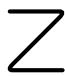
\includegraphics[keepaspectratio]{images/part001_35e3d035.jpg}}

PROPOSITION 2. Let \((\mathfrak{g}_i)_{i\in \mathrm{I}}\) be a finite family of Lie algebras and \(\mathfrak{g} = \prod_{i\in \mathrm{I}}\mathfrak{g}_i\)

The Cartan subalgebras of \(\mathfrak{g}\) are the subalgebras of the form \(\prod_{i\in I}\mathfrak{h}_i\) , where \(\mathfrak{h}_i\) is a Cartan subalgebra of \(\mathfrak{g}_i\) .

If \(h_{i}\) is a subalgebra of \(g_{i}\) with normalizer \(n_{i}\) , then \(\prod h_{i}\) is a subalgebra of g with normalizer \(\prod n_{i}\) ; if the \(h_{i}\) are nilpotent, \(\prod h_{i}\) is nilpotent; thus, if \(h_{i}\) is a Cartan subalgebra of \(g_{i}\) for all i, \(\prod h_{i}\) is a Cartan subalgebra of g. Conversely, let h be a Cartan subalgebra of g; the projection \(h_{i}\) of h onto \(g_{i}\) is a nilpotent subalgebra of \(g_{i}\) , and \(\prod h_{i}\) is a nilpotent subalgebra of g containing h; hence \(h = \prod h_{i}\) (Prop. 1); thus, for all i, \(h_{i}\) is its own normalizer in \(g_{i}\) , and so is a Cartan subalgebra of \(g_{i}\) .

Example 4. If k is of characteristic 0, \(\mathfrak{gl}(n,k)\) is the product of the ideals \(\mathfrak{sl}(n,k)\) and k.1. It follows from Example 2 and Prop. 2 that the set of diagonal matrices of trace 0 in \(\mathfrak{sl}(n,k)\) is a Cartan subalgebra of \(\mathfrak{sl}(n,k)\) .

PROPOSITION 3. Let g be a Lie algebra, h a subalgebra of g, and \(k'\) an extension of k. Then h is a Cartan subalgebra of g if and only if \(h \otimes_{k} k'\) is a Cartan subalgebra of \(g \otimes_{k} k'\) .

Indeed, \(\mathfrak{h}\) is nilpotent if and only if \(\mathfrak{h} \otimes_k k'\) is (Chap. I, §4, no. 5). On the other hand, if \(\mathfrak{n}\) is the normalizer of \(\mathfrak{h}\) in \(\mathfrak{g}\) , the normalizer of \(\mathfrak{h} \otimes_k k'\) in \(\mathfrak{g} \otimes_k k'\) is \(\mathfrak{n} \otimes_k k'\) (Chap. I, §3, no. 8).

PROPOSITION 4. Let \(\mathfrak{g}\) be a Lie algebra, \(\mathfrak{h}\) a nilpotent subalgebra of \(\mathfrak{g}\) . Then \(\mathfrak{h}\) is a Cartan subalgebra of \(\mathfrak{g}\) if and only if \(\mathfrak{g}^0 (\mathfrak{h}) = \mathfrak{h}\) .

If \(\mathfrak{g}^0 (\mathfrak{h}) = \mathfrak{h}\) , \(\mathfrak{h}\) is its own normalizer (§1, Prop. 10 (i)), so \(\mathfrak{h}\) is a Cartan subalgebra of \(\mathfrak{g}\) . Assume that \(\mathfrak{g}^0 (\mathfrak{h})\neq \mathfrak{h}\) . Consider the representation of \(\mathfrak{h}\) on \(\mathfrak{g}^0 (\mathfrak{h}) / \mathfrak{h}\) obtained from the adjoint representation by passage to the quotient. By applying Engel's theorem (Chap. I, §4, no. 2, Th. 1), we see that there exists \(x\in \mathfrak{g}^0 (\mathfrak{h})\) such that \(x\notin \mathfrak{h}\) and \([\mathfrak{h},x]\subset \mathfrak{h}\) ; then \(x\) belongs to the normalizer of \(\mathfrak{h}\) in \(\mathfrak{g}\) , so \(\mathfrak{h}\) is not a Cartan subalgebra of \(\mathfrak{g}\) .

COROLLARY 1. Let \(\mathfrak{g}\) be a Lie algebra, \(\mathfrak{h}\) a Cartan subalgebra of \(\mathfrak{g}\) . If \(k\) is infinite, there exists \(x \in \mathfrak{h}\) such that \(\mathfrak{h} = \mathfrak{g}^0(x)\) .

Indeed, \(\mathfrak{h} = \mathfrak{g}^0 (\mathfrak{h})\) and we can apply Prop. 9 (ii) of §1.

COROLLARY 2. Let \(f: \mathfrak{g} \to \mathfrak{g}'\) be a surjective homomorphism of Lie algebras. If \(\mathfrak{h}\) is a Cartan subalgebra of \(\mathfrak{g}\) , \(f(\mathfrak{h})\) is a Cartan subalgebra of \(\mathfrak{g}'\) .

Indeed, \(f(\mathfrak{h})\) is a nilpotent subalgebra of \(\mathfrak{g}'\) . On the other hand, consider the representation \(x \mapsto \operatorname{ad} f(x)\) of \(\mathfrak{h}\) on \(\mathfrak{g}'\) . By Prop. 9 (iv) of §1, no. 3, \(f(\mathfrak{g}^0(\mathfrak{h})) = \mathfrak{g}'^0(\mathfrak{h})\) . Now \(\mathfrak{g}^0(\mathfrak{h}) = \mathfrak{h}\) , and on the other hand it is clear that \(\mathfrak{g}'^0(\mathfrak{h}) = \mathfrak{g}'^0(f(\mathfrak{h}))\) . Hence, \(f(\mathfrak{h}) = \mathfrak{g}'^0(f(\mathfrak{h}))\) and it suffices to apply Prop. 4.

COROLLARY 3. Let \(\mathfrak{h}\) be a Cartan subalgebra of a Lie algebra \(\mathfrak{g}\) , and let \(\mathcal{C}^n\mathfrak{g}\) ( \(n \geq 1\) ) be a term of the descending central series of \(\mathfrak{g}\) (Chap. I, §1, no. 5). Then \(\mathfrak{g} = \mathfrak{h} + \mathcal{C}^n\mathfrak{g}\) .

Indeed, Corollary 2 shows that the image of \(\mathfrak{h}\) in \(\mathfrak{g} / \mathcal{C}^n\mathfrak{g}\) is a Cartan subalgebra of \(\mathfrak{g} / \mathcal{C}^n\mathfrak{g}\) , hence is equal to \(\mathfrak{g} / \mathcal{C}^n\mathfrak{g}\) since \(\mathfrak{g} / \mathcal{C}^n\mathfrak{g}\) is nilpotent (Example 1).

COROLLARY 4. Let \(\mathfrak{g}\) be a Lie algebra, \(\mathfrak{h}\) a Cartan subalgebra of \(\mathfrak{g}\) , and \(\mathfrak{a}\) a subalgebra of \(\mathfrak{g}\) containing \(\mathfrak{h}\) .

\begin{enumerate}
\def\labelenumi{(\roman{enumi})}
\item
  \(\mathfrak{a}\) is equal to its own normalizer in \(\mathfrak{g}\) .
\item
  Assume that \(k = \mathbf{R}\) or \(\mathbf{C}\) ; let \(G\) be a Lie group with Lie algebra \(\mathfrak{g}\) , A the integral subgroup of \(G\) with Lie algebra \(\mathfrak{a}\) . Then \(A\) is a Lie subgroup of \(G\) , and it is the identity component of the normalizer of \(A\) in \(G\) .
\end{enumerate}

Let n be the normalizer of a in g. Since h is a Cartan subalgebra of n (Example 3), \(\{0\}\) is a Cartan subalgebra of n/a (Cor. 2), hence is equal to its normalizer in n/a; in other words, n = a. Assertion (ii) follows from (i) and Chap. III, §9, no. 4, Cor. of Prop. 11.

COROLLARY 5. Let g be a Lie algebra, E a subset of g. Let E operate on g by the adjoint representation. Then E is a Cartan subalgebra of g if and only if \(E = \mathfrak{g}^{0}(E)\) .

The condition is necessary (Prop. 4). Assume now that \(\mathrm{E} = \mathfrak{g}^0 (\mathrm{E})\) . By Prop. 2 (ii) of §1, no. 1, E is then a subalgebra of \(\mathfrak{g}\) . If \(x\in \mathrm{E}\) , \(\mathrm{ad}_{\mathrm{E}}x\) is nilpotent since \(\mathrm{E}\subset \mathfrak{g}^0 (\mathrm{E})\) ; hence the algebra E is nilpotent. But then E is a Cartan subalgebra by Prop. 4.

COROLLARY 6. Let g be a Lie algebra, let \(k_{0}\) be a subfield of k such that \([k:k_{0}]<+\infty\) , and let \(g_{0}\) be the Lie algebra obtained from g by restricting the field of scalars to \(k_{0}\) . Let h be a subset of g. Then h is a Cartan subalgebra of g if and only if h is a Cartan subalgebra of \(g_{0}\) .

This follows from Cor. 5, since the condition \(\mathfrak{h} = \mathfrak{g}^0 (\mathfrak{h})\) does not involve the base field.

PROPOSITION 5. Let g be a Lie algebra, c its centre, h a vector subspace of g. Then h is a Cartan subalgebra of g if and only if h contains c and h/c is a Cartan subalgebra of g/c.

Assume that \(\mathfrak{h}\) is a Cartan subalgebra of \(\mathfrak{g}\) . Since \([\mathfrak{c},\mathfrak{g}]\subset \mathfrak{h}\) , we have \(\mathfrak{c}\subset \mathfrak{h}\) . On the other hand, \(\mathfrak{h} / \mathfrak{c}\) is a Cartan subalgebra of \(\mathfrak{g} / \mathfrak{c}\) by Cor. 2 of Prop. 4.

Assume that \(\mathfrak{h} \supset \mathfrak{c}\) and that \(\mathfrak{h} / \mathfrak{c}\) is a Cartan subalgebra of \(\mathfrak{g} / \mathfrak{c}\) . Let \(f\) be the canonical morphism from \(\mathfrak{g}\) to \(\mathfrak{g} / \mathfrak{c}\) . The algebra \(\mathfrak{h}\) , which is a central extension of \(\mathfrak{h} / \mathfrak{c}\) , is nilpotent. Let \(\mathfrak{n}\) be the normalizer of \(\mathfrak{h}\) in \(\mathfrak{g}\) . If \(x \in \mathfrak{n}\) , \([f(x), \mathfrak{h} / \mathfrak{c}] \subset \mathfrak{h} / \mathfrak{c}\) , hence \(f(x) \in \mathfrak{h} / \mathfrak{c}\) , and so \(x \in \mathfrak{h}\) . This proves that \(\mathfrak{h}\) is a Cartan subalgebra of \(\mathfrak{g}\) .

COROLLARY. Let \(\mathcal{C}_{\infty}\mathfrak{g}\) be the union of the ascending central series of the Lie algebra \(\mathfrak{g}\) (Chap. I, §1, no. 6). The Cartan subalgebras of \(\mathfrak{g}\) are the inverse images of the Cartan subalgebras of \(\mathfrak{g}/\mathcal{C}_{\infty}\mathfrak{g}\) .

Indeed, the centre of \(\mathfrak{g} / \mathcal{C}_i\mathfrak{g}\) is \(\mathcal{C}_{i + 1}\mathfrak{g} / \mathcal{C}_i\mathfrak{g}\) , and the corollary follows immediately from Prop. 5 by induction.

Remark. \(C_{\infty}g\) is the smallest ideal n of g such that the centre of g/n is zero; it is a characteristic and nilpotent ideal of g.

\subsection{REGULAR ELEMENTS OF A LIE ALGEBRA}

{[}Recall that \(k\) is assumed to be infinite from now on.{]}

Let g be a Lie algebra of dimension n.~If \(x \in g\) , write the characteristic polynomial of ad x in the form

\[
\det (\mathrm{T} - \operatorname{ad} x) = \sum_ {i = 0} ^ {n} a _ {i} (x) \mathrm{T} ^ {i}, \quad \text { with } a _ {i} (x) \in k.
\]

We have \(a_i(x) = (-1)^{n - i}\mathrm{Tr}\left(\bigwedge^{n - i}\operatorname {ad}x\right)\) , cf.~Algebra, Chap. III, §8, no. 11. This shows that \(x\mapsto a_i(x)\) is a homogeneous polynomial map of degree \(n - i\) from \(\mathfrak{g}\) to \(k\) (Algebra, Chap. IV, §5, no. 9).

Remarks. 1) If \(\mathfrak{g} \neq \{0\}\) , \(a_0 = 0\) since (ad \(x(x) = 0\) for all \(x \in \mathfrak{g}\) .

\begin{enumerate}
\def\labelenumi{\arabic{enumi})}
\setcounter{enumi}{1}
\tightlist
\item
  Let \(k'\) be an extension of \(k\) . Write \(\det(\mathrm{T} - \operatorname{ad} x') = \sum_{i=0}^{n} a_i'(x') \mathrm{T}^i\) for \(x' \in \mathfrak{g} \otimes_k k'\) . Then \(a_i'| \mathfrak{g} = a_i\) for all \(i\) .
\end{enumerate}

DEFINITION 2. The rank of g, denoted by rk(g), is the smallest integer l such that \(a_{l} \neq 0\) . An element x of g is called regular if \(a_{l}(x) \neq 0\) .

For all \(x \in \mathfrak{g}\) , \(\operatorname{rk}(\mathfrak{g}) \leq \dim \mathfrak{g}^0(x)\) , and equality holds if and only if \(x\) is regular.

The set of regular elements is dense and open in \(\mathfrak{g}\) for the Zariski topology (App. I).

Examples. 1) If g is nilpotent, rk(g) = dim g and all elements of g are regular.

\begin{enumerate}
\def\labelenumi{\arabic{enumi})}
\setcounter{enumi}{1}
\tightlist
\item
  Let \(\mathfrak{g} = \mathfrak{sl}(2,k)\) . If \(x = \begin{pmatrix} \gamma & \alpha \\ \beta & -\gamma \end{pmatrix} \in \mathfrak{g}\) , an easy calculation gives
\end{enumerate}

\[
\det (\mathrm{T} - \operatorname{ad} x) = \mathrm{T} ^ {3} - 4 (\alpha \beta + \gamma^ {2}) \mathrm{T}.
\]

If the characteristic of \(k\) is \(\neq 2\) , then \(\mathrm{rk}(\mathfrak{g}) = 1\) and the regular elements are those \(x\) such that \(\alpha \beta + \gamma^2 \neq 0\) .

\begin{enumerate}
\def\labelenumi{\arabic{enumi})}
\setcounter{enumi}{2}
\tightlist
\item
  Let V be a vector space of finite dimension n, and \(\mathfrak{g} = \mathfrak{gl}(V)\) . Let \(\overline{k}\) be an algebraic closure of k. Let \(x \in g\) , and let \(\lambda_{1}, \ldots, \lambda_{n}\) be the roots in \(\overline{k}\) of the characteristic polynomial of x (each root being written a number of times equal to its multiplicity). The canonical isomorphism from \(V^{*} \otimes V\) to g is compatible with the g-module structures of these two spaces, in other words it takes \(1 \otimes x - {}^{t}x \otimes 1\) to ad x (Chap. I, §3, no. 3, Prop. 4). In view of §1, Prop. 4 (i), it follows that the roots of the characteristic polynomial of ad x are the \(\lambda_{i} - \lambda_{j}\) for \(1 \leq i \leq n, 1 \leq j \leq n\) (each root being written a number of times equal to its multiplicity). Thus, the rank of g is n, and x is regular if and only if each \(\lambda_{i}\) is a simple root of the characteristic polynomial of x.
\end{enumerate}

PROPOSITION 6. Let \(\mathfrak{g}\) be a Lie algebra, \(k'\) an extension of \(k\) , and \(\mathfrak{g}' = \mathfrak{g} \otimes_k k'\) .

\begin{enumerate}
\def\labelenumi{(\roman{enumi})}
\tightlist
\item
  An element \(x\) of \(\mathfrak{g}\) is regular in \(\mathfrak{g}\) if and only if \(x \otimes 1\) is regular in \(\mathfrak{g}'\) .\\
\item
  \(\operatorname{rk}(\mathfrak{g}) = \operatorname{rk}(\mathfrak{g}')\) .
\end{enumerate}

This follows from Remark 2.

PROPOSITION 7. Let \((\mathfrak{g}_i)_{i\in \mathrm{I}}\) be a finite family of Lie algebras, and let \(\mathfrak{g} = \prod_{i\in \mathrm{I}}\mathfrak{g}_i\) .

\begin{enumerate}
\def\labelenumi{(\roman{enumi})}
\tightlist
\item
  An element \((x_{i})_{i\in \mathrm{I}}\) of \(\mathfrak{g}\) is regular in \(\mathfrak{g}\) if and only if, for all \(i\in \mathrm{I}\) , \(x_{i}\) is regular in \(\mathfrak{g}_i\) .
\end{enumerate}

\[
\text {(ii)} \operatorname{rk} (\mathfrak {g}) = \sum_ {i \in I} \operatorname{rk} (\mathfrak {g} _ {i}).
\]

Indeed, for any \(x = (x_{i})_{i \in \mathrm{I}} \in \mathfrak{g}\) , the characteristic polynomial of \(ad_{g}x\) is the product of the characteristic polynomials of the \(ad_{g_{i}}x_{i}\) .

PROPOSITION 8. Let \(f: \mathfrak{g} \to \mathfrak{g}'\) be a surjective homomorphism of Lie algebras.

\begin{enumerate}
\def\labelenumi{(\roman{enumi})}
\item
  If \(x\) is a regular element of \(\mathfrak{g}\) , \(f(x)\) is regular in \(\mathfrak{g}'\) . The converse is true if \(\operatorname{Ker} f\) is contained in the centre of \(\mathfrak{g}\) .
\item
  \(\operatorname{rk}(\mathfrak{g}) \geq \operatorname{rk}(\mathfrak{g}')\) .
\end{enumerate}

Put \(\mathrm{rk}(\mathfrak{g}) = r, \mathrm{rk}(\mathfrak{g}') = r'\) . Let \(x \in \mathfrak{g}\) . The characteristic polynomials of \(\operatorname{ad} x\) , \(\operatorname{ad} f(x)\) and \(\operatorname{ad} x|\operatorname{Ker} f\) are of the form

\[
\mathrm{P} (\mathrm{T}) = \mathrm{T} ^ {n} + a _ {n - 1} (x) \mathrm{T} ^ {n - 1} + \dots + a _ {r} (x) \mathrm{T} ^ {r},
\]

\[
\mathrm{Q} (\mathrm{T}) = \mathrm{T} ^ {n ^ {\prime}} + b _ {n ^ {\prime} - 1} (x) \mathrm{T} ^ {n ^ {\prime} - 1} + \dots + b _ {r ^ {\prime}} (x) \mathrm{T} ^ {r ^ {\prime}},
\]

\[
\mathrm{R} (\mathrm{T}) = \mathrm{T} ^ {n ^ {\prime \prime}} + c _ {n ^ {\prime \prime} - 1} (x) \mathrm{T} ^ {n ^ {\prime \prime} - 1} + \dots + c _ {r ^ {\prime \prime}} (x) \mathrm{T} ^ {r ^ {\prime \prime}},
\]

where the \(a_i, b_i, c_i\) are polynomial functions on \(\mathfrak{g}\) , with \(a_r \neq 0\) , \(b_{r'} \neq 0\) , \(c_{r''} \neq 0\) . We have \(\mathrm{P} = \mathrm{QR}\) , so \(r = r' + r''\) and \(a_r(x) = b_{r'}(x)c_{r''}(x)\) , which proves (ii) and the first assertion of (i). If \(\operatorname{Ker} f\) is contained in the centre of \(\mathfrak{g}\) , \(\mathrm{R(T)} = \mathrm{T}^{n''}\) and so \(a_r(x) = b_{r'}(x)\) , hence the second assertion of (i).

COROLLARY. Let \(\mathcal{C}_n\mathfrak{g}\) ( \(n \geq 0\) ) be a term of the ascending central series of \(\mathfrak{g}\) (Chap. I, §1, no. 6). The regular elements of \(\mathfrak{g}\) are those whose image in \(\mathfrak{g}/\mathcal{C}_n\mathfrak{g}\) is regular.

PROPOSITION 9. Let \(\mathfrak{g}\) be a Lie algebra, \(\mathfrak{g}'\) a subalgebra of \(\mathfrak{g}\) . Every element of \(\mathfrak{g}'\) regular in \(\mathfrak{g}\) is regular in \(\mathfrak{g}'\) .

For \(x \in g'\) , the restriction of \(ad_{g}x\) to \(g'\) is \(ad_{g'}x\) , and so defines an endomorphism \(u(x)\) of the vector space \(g/g'\) by passage to the quotient. Let \(d_{0}(x)\) (resp. \(d_{1}(x)\) ) be the dimension of the nilspace of \(ad_{g'}(x)\) (resp. of \(u(x)\) ), and let \(c_{0}\) (resp. \(c_{1}\) ) be the minimum of \(d_{0}(x)\) (resp. \(d_{1}(x)\) ) when x belongs to \(g'\) . There exist non-zero polynomial maps \(p_{0}, p_{1}\) from \(g'\) to k such that

\[
d _ {0} (x) = c _ {0} \Longleftrightarrow p _ {0} (x) \neq 0, \quad d _ {1} (x) = c _ {1} \Longleftrightarrow p _ {1} (x) \neq 0.
\]

Since k is infinite, the set S of \(x \in g'\) such that \(d_{0}(x) = c_{0}\) and \(d_{1}(x) = c_{1}\) is non-empty. Every element of S is regular in \(g'\) . On the other hand, S is the set of elements of \(g'\) such that the nilspace of \(ad_{g}x\) has minimum dimension, and thus contains every element of \(g'\) regular in g.

Remark. 3) Elements of \(\mathfrak{g}'\) regular in \(\mathfrak{g}\) do not necessarily exist. If at least one does exist, the set of these elements is precisely the set denoted by S in the above proof.

\subsection{CARTAN SUBALGEBRAS AND REGULAR ELEMENTS}

THEOREM 1. Let \(\mathfrak{g}\) be a Lie algebra.

\begin{enumerate}
\def\labelenumi{(\roman{enumi})}
\item
  If \(x\) is a regular element of \(\mathfrak{g}\) , \(\mathfrak{g}^0(x)\) is a Cartan subalgebra of \(\mathfrak{g}\) .
\item
  If \(\mathfrak{h}\) is a maximal nilpotent subalgebra of \(\mathfrak{g}\) , and if \(x \in \mathfrak{h}\) is regular in \(\mathfrak{g}\) , then \(\mathfrak{h} = \mathfrak{g}^0(x)\) .
\item
  If \(\mathfrak{h}\) is a Cartan subalgebra of \(\mathfrak{g}\) , then \(\dim (\mathfrak{h})\geq \mathrm{rk}(\mathfrak{g})\)
\item
  The Cartan subalgebras of \(\mathfrak{g}\) of dimension \(\mathrm{rk}(\mathfrak{g})\) are the \(\mathfrak{g}^0 (x)\) where \(x\) is a regular element.
\end{enumerate}

Let \(x\) be a regular element of \(\mathfrak{g}\) and let \(\mathfrak{h} = \mathfrak{g}^0(x)\) . Clearly \(\mathfrak{h}^0(x) = \mathfrak{h}\) . Since \(x\) is regular in \(\mathfrak{h}\) (Prop. 9), \(\operatorname{rk}(\mathfrak{h}) = \dim(\mathfrak{h})\) , so \(\mathfrak{h}\) is nilpotent. On the other hand, \(\mathfrak{h} = \mathfrak{g}^0(x) \supset \mathfrak{g}^0(\mathfrak{h}) \supset \mathfrak{h}\) , so \(\mathfrak{h} = \mathfrak{g}^0(\mathfrak{h})\) is a Cartan subalgebra of \(\mathfrak{g}\) (Prop. 4). This proves (i).

If \(\mathfrak{h}\) is a maximal nilpotent subalgebra of \(\mathfrak{g}\) , and if \(x\in \mathfrak{h}\) is regular in \(\mathfrak{g}\) , then \(\mathfrak{h}\subset \mathfrak{g}^0 (x)\) and \(\mathfrak{g}^0 (x)\) is nilpotent by (i), so \(\mathfrak{h} = \mathfrak{g}^0 (x)\) , which proves (ii).

If \(\mathfrak{h}\) is a Cartan subalgebra of \(\mathfrak{g}\) , there exists \(x \in \mathfrak{h}\) such that \(\mathfrak{h} = \mathfrak{g}^0(x)\) (Cor. 1 of Prop. 4), so \(\dim(\mathfrak{h}) \geq \operatorname{rk}(\mathfrak{g})\) , which proves (iii). If in addition \(\dim(\mathfrak{h}) = \operatorname{rk}(\mathfrak{g})\) , \(x\) is regular. Finally, if \(x'\) is regular in \(\mathfrak{g}\) , \(\mathfrak{g}^0(x')\) is a Cartan subalgebra by (i), and is obviously of dimension \(\operatorname{rk}(\mathfrak{g})\) . This proves (iv).

We shall see in §3, Th. 2 that, when \(k\) is of characteristic zero, all the Cartan subalgebras of \(\mathfrak{g}\) have dimension \(\mathrm{rk}(\mathfrak{g})\) .

COROLLARY 1. Every Lie algebra g has Cartan subalgebras, and the rank of g is the minimum dimension of a Cartan subalgebra.

COROLLARY 2. Let \(f: \mathfrak{g} \to \mathfrak{g}'\) be a surjective homomorphism of Lie algebras. If \(\mathfrak{h}'\) is a Cartan subalgebra of \(\mathfrak{g}'\) , there exists a Cartan subalgebra \(\mathfrak{h}\) of \(\mathfrak{g}\) such that \(\mathfrak{h}' = f(\mathfrak{h})\) .

Let \(\mathfrak{a} = f^{-1}(\mathfrak{h}')\) . By Cor. 1, \(\mathfrak{a}\) has a Cartan subalgebra \(\mathfrak{h}\) . By Cor. 2 of Prop. 4, \(f(\mathfrak{h}) = \mathfrak{h}'\) . We show that \(\mathfrak{h}\) is a Cartan subalgebra of \(\mathfrak{g}\) . Let \(\mathfrak{n}\) be the normalizer of \(\mathfrak{h}\) in \(\mathfrak{g}\) . It is enough to prove that \(\mathfrak{h} = \mathfrak{n}\) . If \(x \in \mathfrak{n}\) , \(f(x)\) belongs to the normalizer of \(\mathfrak{h}'\) in \(\mathfrak{g}'\) , so \(f(x) \in \mathfrak{h}'\) and \(x \in \mathfrak{a}\) ; but \(\mathfrak{h}\) is its own normalizer in \(\mathfrak{a}\) , so \(x \in \mathfrak{h}\) .

COROLLARY 3. Every Lie algebra \(\mathfrak{g}\) is the sum of its Cartan subalgebras.

The sum s of the Cartan subalgebras of g contains the set of regular elements of g (Th. 1 (i)). Since this set is dense in g for the Zariski topology, s = g.

PROPOSITION 10. Let g be a Lie algebra, a a commutative subalgebra of g and c the commutant of a in g. Assume that \(ad_{g}x\) is semi-simple for all \(x \in a\) . Then the Cartan subalgebras of c are the Cartan subalgebras of g containing a.

Let \(\mathfrak{h}\) be a Cartan subalgebra of \(\mathfrak{c}\) . Since \(\mathfrak{a}\) is contained in the centre \(\mathfrak{z}\) of \(\mathfrak{c}, \mathfrak{a} \subset \mathfrak{z} \subset \mathfrak{h}\) (Prop. 5). Let \(\mathfrak{n}\) be the normalizer of \(\mathfrak{h}\) in \(\mathfrak{g}\) . Then

\[
[ \mathfrak {a}, \mathfrak {n} ] \subset [ \mathfrak {h}, \mathfrak {n} ] \subset \mathfrak {h}.
\]

Since the \(ad_{g}x\) , \(x \in a\) , are semi-simple and commute with each other, it follows from Algebra, Chap. VIII, §5, no. 1, that there exists a vector subspace d of n stable under \(ad_{g}a\) and such that \(n = h \oplus d\) . Then \([a, d] \subset h \cap d = 0\) , so \(d \subset c\) . Thus, n is the normalizer of h in c, and hence \(n = h\) , so h is a Cartan subalgebra of g containing a.

Conversely, let \(\mathfrak{h}\) be a Cartan subalgebra of \(\mathfrak{g}\) containing \(\mathfrak{a}\) . Then \(\mathfrak{h} = \mathfrak{g}^0 (\mathfrak{h})\subset \mathfrak{g}^0 (\mathfrak{a})\) , and by hypothesis \(\mathfrak{g}_0(\mathfrak{a}) = \mathfrak{g}^0 (\mathfrak{a}) = \mathfrak{c}\) . Hence \(\mathfrak{a}\subset \mathfrak{h}\subset \mathfrak{c}\) and \(\mathfrak{h}\) is a Cartan subalgebra of \(\mathfrak{c}\) (for it is equal to its own normalizer in \(\mathfrak{g}\) , and so a fortiori in \(\mathfrak{c}\) ).

PROPOSITION 11. Let \(\mathfrak{n}\) be a nilpotent subalgebra of a Lie algebra \(\mathfrak{g}\) . There exists a Cartan subalgebra of \(\mathfrak{g}\) contained in \(\mathfrak{g}^0 (\mathfrak{n})\) .

Put \(\mathfrak{a} = \mathfrak{g}^0 (\mathfrak{n})\) . Then \(\mathfrak{n}\subset \mathfrak{a}\) since \(\mathfrak{n}\) is nilpotent. If \(x\in \mathfrak{a}\) , let \(\mathrm{P}(x)\) be the determinant of the endomorphism of \(\mathfrak{g} / \mathfrak{a}\) defined by ad \(x\) . Denote by \(\mathfrak{a}'\) the set of \(x\in \mathfrak{a}\) such that \(\mathrm{P}(x)\neq 0\) , which is an open subset of \(\mathfrak{a}\) in the Zariski topology; the relations \(x\in \mathfrak{a}'\) and \(\mathfrak{g}^0 (x)\subset \mathfrak{a}\) are equivalent. By Prop. 7 (ii) of §1, no. 2, there exists \(y\in \mathfrak{n}\) such that \(\mathfrak{g}^0 (y) = \mathfrak{a}\) , and \(y\in \mathfrak{a}'\) so \(\mathfrak{a}'\) is non-empty. Since \(\mathfrak{a}'\) is open, its intersection with the set of regular elements of \(\mathfrak{a}\) is non-empty. Let \(x\) be an element of this intersection. Then \(\mathfrak{g}^0 (x)\subset \mathfrak{a}\) and \(\mathfrak{g}^0 (x)\) is a Cartan subalgebra of \(\mathfrak{a}\) , hence is nilpotent. On the other hand, Prop. 10 (i) of §1, no. 3, shows that \(\mathfrak{g}^0 (x)\) is its own normalizer in \(\mathfrak{g}\) ; it is therefore a Cartan subalgebra of \(\mathfrak{g}\) , which completes the proof.

\subsection{CARTAN SUBALGEBRAS OF SEMI-SIMPLE LIE ALGEBRAS}

THEOREM 2. Assume that k is of characteristic 0. Let g be a semi-simple Lie algebra, h a Cartan subalgebra of g. Then h is commutative, and all of its elements are semi-simple in g (Chap. I, §6, no. 3, Def. 3).

Since \(\mathfrak{h} = \mathfrak{g}^0 (\mathfrak{h})\) , \(\mathfrak{h}\) is reductive (§1, Prop. 11), hence commutative since it is nilpotent. On the other hand, the restriction of the adjoint representation of \(\mathfrak{g}\) to \(\mathfrak{h}\) is semi-simple (loc. cit.), so the elements of \(\mathfrak{h}\) are semi-simple in \(\mathfrak{g}\) (Algebra, Chap. VIII, §5, no. 1).

COROLLARY 1. If \(x \in \mathfrak{h}\) and \(y \in \mathfrak{g}^{\lambda}(\mathfrak{h})\) , we have \([x, y] = \lambda(x)y\) .

Indeed, \(\mathfrak{g}^{\lambda (x)}(x) = \mathfrak{g}_{\lambda (x)}(x)\) since ad \(x\) is semi-simple.

COROLLARY 2. Every regular element of g is semi-simple.

Indeed, such an element belongs to a Cartan subalgebra (no. 3, Th. 1 (i)).

COROLLARY 3. Let \(\mathfrak{h}\) be a Cartan subalgebra of a reductive Lie algebra \(\mathfrak{g}\) . a) \(\mathfrak{h}\) is commutative.

\begin{enumerate}
\def\labelenumi{\alph{enumi})}
\setcounter{enumi}{1}
\tightlist
\item
  If \(\rho\) is a finite dimensional semi-simple representation of \(\mathfrak{g}\) , the elements of \(\rho(\mathfrak{h})\) are semi-simple.
\end{enumerate}

Let \(\mathfrak{c}\) be the centre of \(\mathfrak{g}\) , and \(\mathfrak{s}\) its derived algebra. Then \(\mathfrak{g} = \mathfrak{c} \times \mathfrak{s}\) , so \(\mathfrak{h} = \mathfrak{c} \times \mathfrak{h}'\) , where \(\mathfrak{h}'\) is a Cartan subalgebra of \(\mathfrak{s}\) (Prop. 2). In view of Th. 2, \(\mathfrak{h}'\) is commutative, hence so is \(\mathfrak{h}\) . Moreover, \(\rho(\mathfrak{h}')\) consists of semi-simple elements and so does \(\rho(\mathfrak{c})\) (Chap. I, §6, no. 5, Th. 4); assertion \(b\) ) follows.

\section{CONJUGACY THEOREMS}

In this paragraph, the base field \(k\) is of characteristic 0.

\subsection{ELEMENTARY AUTOMORPHISMS}

Let \(\mathfrak{g}\) be a Lie algebra. Denote its group of automorphisms by \(\operatorname{Aut}(\mathfrak{g})\) . If \(x \in \mathfrak{g}\) and if \(\operatorname{ad} x\) is nilpotent, \(e^{\operatorname{ad} x} \in \operatorname{Aut}(\mathfrak{g})\) (Chap. I, §6, no. 8).

DEFINITION 1. A finite product of automorphisms of g of the form \(e^{ad x}\) with ad x nilpotent is called an elementary automorphism of g. The group of elementary automorphisms of g is denoted by \(\operatorname{Aut}_{e}(\mathfrak{g})\) .

If \(u \in \operatorname{Aut}(\mathfrak{g})\) , \(ue^{\operatorname{ad}x}u^{-1} = e^{\operatorname{ad}u(x)}\) . It follows that \(\operatorname{Aut}_{e}(\mathfrak{g})\) is a normal subgroup of \(\operatorname{Aut}(\mathfrak{g})\) . If k = R or C, \(\operatorname{Aut}_{e}(\mathfrak{g})\) is contained in the group \(\operatorname{Int}(\mathfrak{g})\) of inner automorphisms of g (Chap. III, §6, no. 2, Def. 2).

* In the general case, \(\mathrm{Aut}_e(\mathfrak{g})\) is contained in the identity component of the algebraic group \(\mathrm{Aut}(\mathfrak{g})\) .*

Lemma 1. Let \(\mathrm{V}\) be a finite dimensional vector space, \(\mathfrak{n}\) a Lie subalgebra of \(\mathfrak{a} = \mathfrak{gl}(\mathrm{V})\) consisting of nilpotent elements.

\begin{enumerate}
\def\labelenumi{(\roman{enumi})}
\item
  The map \(x \mapsto \exp x\) is a bijection from \(\mathfrak{n}\) to a subgroup \(N\) of \(\mathbf{GL}(V)\) consisting of unipotent elements (Chap. II, §6, no. 1, Remark 4). We have \(\mathfrak{n} = \log(\exp \mathfrak{n})\) . The map \(f \mapsto f \circ \log\) is an isomorphism from the algebra of polynomial functions on \(\mathfrak{n}\) to the algebra of restrictions to \(\mathbf{N}\) of polynomial functions on \(\operatorname{End}(\mathbf{V})\) .
\item
  If \(x \in \mathfrak{n}\) and \(a \in \mathfrak{a}\) ,
\end{enumerate}

\[
(\exp \operatorname{ad} _ {\mathfrak {a}} x). a = (\exp x) a (\exp (- x)).
\]

\begin{enumerate}
\def\labelenumi{(\roman{enumi})}
\setcounter{enumi}{2}
\tightlist
\item
  Let \(V'\) be a finite dimensional vector space, \(n'\) a Lie subalgebra of \(\mathfrak{gl}(V')\) consisting of nilpotent elements, \(\rho\) a homomorphism from n to \(n'\) . Let \(\pi\) be the map \(\exp x \mapsto \exp \rho(x)\) from \(\exp n\) to \(\exp n'\) . Then \(\pi\) is a group homomorphism.
\end{enumerate}

By Engel's theorem, we can identify V with \(k^n\) in such a way that \(\mathfrak{n}\) is a subalgebra of \(\mathfrak{n}(n,k)\) (the Lie subalgebra of \(\mathbf{M}_n(k)\) consisting of the lower triangular matrices with zeros on the diagonal). For \(s \geq 0\) , let \(\mathfrak{n}_s(n,k)\) be the set of \((x_{ij})_{1 \leq i,j \leq n} \in \mathbf{M}_n(k)\) such that \(x_{ij} = 0\) for \(i - j < s\) . Then

\[
[ \mathfrak {n} _ {s} (n, k), \mathfrak {n} _ {s ^ {\prime}} (n, k) ] \subset \mathfrak {n} _ {s + s ^ {\prime}} (n, k)
\]

(Chap. II, §4, no. 6, Remark), and the Hausdorff series defines a polynomial map \((a,b)\mapsto\mathrm{H}(a,b)\) from \(\mathfrak{n}(n,k)\times\mathfrak{n}(n,k)\) to \(\mathfrak{n}(n,k)\) (Chap. II, §6, no. 5, Remark 3); this map makes \(\mathfrak{n}(n,k)\) into a group (Chap. II, §6, no. 5, Prop. 4). By Chap. II, §6, no. 1, Remark 4, the maps \(x\mapsto\exp x\) from \(\mathfrak{n}(n,k)\) to \(1+\mathfrak{n}(n,k)\) and \(y\mapsto\log y\) from \(1+\mathfrak{n}(n,k)\) to \(\mathfrak{n}(n,k)\) are inverse bijections and are polynomial; by Chap. II, §6, no. 5, Prop. 3, these maps are isomorphisms of groups if \(\mathfrak{n}(n,k)\) is given the group law \((a,b)\mapsto\mathrm{H}(a,b)\) and if \(1+\mathfrak{n}(n,k)\) is considered as a subgroup of \(\mathbf{GL}_{n}(k)\) . Assertions (i) and (iii) of the lemma now follow. Let \(x\in\mathfrak{n}\) . Denote by \(\mathrm{L}_{x},\mathrm{R}_{x}\) the maps \(u\mapsto xu,u\mapsto ux\) from \(\mathfrak{a}\) to \(\mathfrak{a}\) , which commute and are nilpotent. We have \(\mathrm{ad}_{\mathfrak{a}}x=\mathrm{L}_{x}-\mathrm{R}_{x}\) , so, for all \(a\in\mathfrak{a}\) ,

\[
\begin{array}{c} (\exp \operatorname{ad} _ {\mathfrak {a}} x) a = (\exp (\mathrm{L} _ {x} - \mathrm{R} _ {x})) a = (\exp \mathrm{L} _ {x}) (\exp \mathrm{R} _ {- x}) a \\ = \sum_ {i, j \geq 0} \frac {\mathrm{L} _ {x} ^ {i}}{i !} \frac {\mathrm{R} _ {- x} ^ {j}}{j !} a = (\exp x) a (\exp (- x)). \end{array}\tag{1}
\]

With the notation in Lemma 1, \(\pi\) is called the linear representation of \(\exp \mathfrak{n}\) compatible with the given representation \(\rho\) of \(\mathfrak{n}\) on \(V'\) . When \(k\) is \(\mathbf{R}\) , \(\mathbf{C}\) , or a non-discrete complete ultrametric field, \(\rho = L(\pi)\) by the properties of exponential maps (Chap. III, §4, no. 4, Cor. 2 of Prop. 8).

PROPOSITION 1. Let \(\mathfrak{g}\) be a Lie algebra, \(\mathfrak{n}\) a subalgebra of \(\mathfrak{g}\) such that \(\operatorname{ad}_{\mathfrak{g}}x\) is nilpotent for all \(x\in \mathfrak{n}\) . Then \(e^{\operatorname{ad}_{\mathfrak{g}}\mathfrak{n}}\) is a subgroup of \(\operatorname{Aut}_e(\mathfrak{g})\) .

This follows immediately from Lemma 1 (i).

In particular, if \(\mathfrak{n}\) is the nilpotent radical of \(\mathfrak{g}\) , \(e^{\mathrm{ad}_{\mathfrak{g}}\mathfrak{n}}\) is the group of special automorphisms of \(\mathfrak{g}\) (Chap. I, §6, no. 8, Def. 6).

Remarks. 1) Let V be a finite dimensional vector space, g a Lie subalgebra of \(\mathfrak{a} = \mathfrak{gl}(V)\) , x an element of g such that \(ad_{g}x\) is nilpotent. Then there exists a nilpotent element n of a such that \(ad_{a}n\) extends \(ad_{g}x\) . Indeed, let s, n be the semi-simple and nilpotent components of x; then \(ad_{a}s\) and \(ad_{a}n\) are the semi-simple and nilpotent components of \(ad_{a}x\) (Chap. I, §5, no. 4, Lemma 2), so \(ad_{a}s\) and \(ad_{a}n\) leave g stable, and \(ad_{a}s|g\) and \(ad_{a}n|g\) are the semi-simple and nilpotent components of \(ad_{g}x\) ; consequently, \(ad_{g}x = ad_{a}n|g\) , which proves our assertion. In view of Lemma 1 (ii), every elementary automorphism of g extends to an automorphism of a of the form \(u \mapsto mum^{-1}\) where \(m \in \mathbf{GL}(V)\) .

\begin{enumerate}
\def\labelenumi{\arabic{enumi})}
\setcounter{enumi}{1}
\tightlist
\item
  Let V be a finite dimensional vector space. For all \(g \in \mathbf{SL}(V)\) , let \(\varphi(g)\) be the automorphism \(x \mapsto gxg^{-1}\) of \(\mathfrak{gl}(V)\) . Then
\end{enumerate}

\[
\operatorname{Aut} _ {e} (\mathfrak {g l} (V)) = \varphi (\mathbf {S L} (V)).
\]

Indeed, by (1), \(\operatorname{Aut}_{e}(\mathfrak{gl}(V))\) is contained in \(\varphi(\mathbf{SL}(V))\) , and the opposite inclusion follows from Algebra, Chap. III, §8, no. 9, Prop. 17 and (1). An analogous argument shows that \(\operatorname{Aut}_{e}(\mathfrak{sl}(V))\) is the set of restrictions of elements of \(\varphi(\mathbf{SL}(V))\) to \(\mathfrak{sl}(V)\) .

\subsection{CONJUGACY OF CARTAN SUBALGEBRAS}

Let g be a Lie algebra, h a nilpotent subalgebra of g and R the set of non-zero weights of h in g, in other words the set of linear forms \(\lambda \neq 0\) on h such that \(\mathfrak{g}^{\lambda}(\mathfrak{h}) \neq 0\) , cf.~§1, no. 3, Prop. 9 (iii). Assume that

\[
\mathfrak {g} = \mathfrak {g} ^ {0} (\mathfrak {h}) \oplus \sum_ {\lambda \in R} \mathfrak {g} ^ {\lambda} (\mathfrak {h}),
\]

which is the case if \(k\) is algebraically closed (§1, no. 3, Prop. 9 (i)). For \(\lambda \in \mathbb{R}\) and \(x \in \mathfrak{g}^{\lambda}(\mathfrak{h})\) , ad \(x\) is nilpotent (§1, no. 3, Prop. 10 (iv)). Denote by \(\mathrm{E}(\mathfrak{h})\) the subgroup of \(\mathrm{Aut}_e(\mathfrak{g})\) generated by the \(e^{\mathrm{ad}x}\) where \(x\) is of the form above. If \(u \in \mathrm{Aut}(\mathfrak{g})\) , it is immediate that \(u\mathrm{E}(\mathfrak{h})u^{-1} = \mathrm{E}(u(\mathfrak{h}))\) .

Lemma 2. (i) Let \(\mathfrak{h}_r\) be the set of \(x\in \mathfrak{h}\) such that \(\mathfrak{g}^0 (x) = \mathfrak{g}^0 (\mathfrak{h})\) ; this is the set of \(x\in \mathfrak{h}\) such that \(\lambda (x)\neq 0\) for all \(\lambda \in \mathrm{R}\) , and \(\mathfrak{h}_r\) is open and dense in \(\mathfrak{h}\) in the Zariski topology.

\begin{enumerate}
\def\labelenumi{(\roman{enumi})}
\setcounter{enumi}{1}
\tightlist
\item
  Put \(R = \{\lambda_{1}, \lambda_{2}, \ldots, \lambda_{p}\}\) where the \(\lambda_{i}\) are mutually distinct. Let F be the map from \(\mathfrak{g}^{0}(\mathfrak{h}) \times \mathfrak{g}^{\lambda_{1}}(\mathfrak{h}) \times \cdots \times \mathfrak{g}^{\lambda_{p}}(\mathfrak{h})\) to g defined by the formula
\end{enumerate}

\[
\mathrm{F} (h, x _ {1}, \dots , x _ {p}) = e ^ {\operatorname{ad} x _ {1}} \dots e ^ {\operatorname{ad} x _ {p}} h.
\]

Then \(\mathrm{F}\) is a dominant polynomial map (App. I).

Assertion (i) is clear. We prove (ii). Let \(n = \dim \mathfrak{g}\) . If \(\lambda \in \mathrm{R}\) and \(x \in \mathfrak{g}^{\lambda}(\mathfrak{h})\) , we have \((\operatorname{ad} x)^n = 0\) . It follows that \((y, x) \mapsto e^{\operatorname{ad} x} y\) is a polynomial map from \(\mathfrak{g} \times \mathfrak{g}^{\lambda}(\mathfrak{h})\) to \(\mathfrak{g}\) ; it follows by induction that \(\mathrm{F}\) is polynomial. Let \(h_0 \in \mathfrak{h}_r\) and let \(\mathrm{DF}\) be the tangent linear map of \(\mathrm{F}\) at \((h_0, 0, \ldots, 0)\) ; we show that \(\mathrm{DF}\) is surjective. For \(h \in \mathfrak{g}^{0}(\mathfrak{h})\) , \(F(h_{0} + h, 0, \ldots, 0) = h_{0} + h\) , so \(\mathrm{DF}(h, 0, \ldots, 0) = h\) and \(\mathrm{Im}(\mathrm{DF}) \supset \mathfrak{g}^{0}(\mathfrak{h})\) . On the other hand, for \(x \in \mathfrak{g}^{\lambda_{1}}(\mathfrak{h})\) ,

\[
\mathrm{F} (h _ {0}, x, 0, \dots , 0) = e ^ {\operatorname{ad} x} h _ {0} = h _ {0} + (\operatorname{ad} x). h _ {0} + \frac {(\operatorname{ad} x) ^ {2}}{2 !} h _ {0} + \dots
\]

so \(\mathrm{DF}(0,x,0,\ldots ,0) = (\mathrm{ad}x).h_0 = -(\mathrm{ad}h_0)x\) ; since \(\mathrm{ad}h_0\) induces an automorphism of \(\mathfrak{g}^{\lambda_1}(\mathfrak{h})\) , \(\operatorname {Im}(\mathrm{DF})\supset \mathfrak{g}^{\lambda_1}(\mathfrak{h})\) . Similarly,

\[
\operatorname{Im} (\mathrm{DF}) \supset \mathfrak {g} ^ {\lambda_ {i}} (\mathfrak {h})
\]

for all \(i\) , hence the surjectivity of DF. Prop. 4 of App. I now shows that F is dominant.

PROPOSITION 2. Assume that \(k\) is algebraically closed. Let \(\mathfrak{g}\) be a Lie algebra, \(\mathfrak{h}\) and \(\mathfrak{h}'\) Cartan subalgebras of \(\mathfrak{g}\) . There exist \(u \in \mathrm{E}(\mathfrak{h})\) and \(u' \in \mathrm{E}(\mathfrak{h}')\) such that \(u(\mathfrak{h}) = u'(\mathfrak{h}')\) .

We retain the notation of Lemma 2. From the fact that \(\mathfrak{h}\) and \(\mathfrak{h}'\) are Cartan subalgebras, it follows that \(\mathfrak{g}^0 (\mathfrak{h}) = \mathfrak{h}\) and \(\mathfrak{g}^0 (\mathfrak{h}') = \mathfrak{h}'\) . By Lemma 2 and Prop. 3 of App. I, \(\mathrm{E}(\mathfrak{h})\mathfrak{h}_r\) and \(\mathrm{E}(\mathfrak{h}')\mathfrak{h}_r'\) contain open dense subsets of \(\mathfrak{g}\) in the Zariski topology. Thus \(\mathrm{E}(\mathfrak{h})\mathfrak{h}_r\cap \mathrm{E}(\mathfrak{h}')\mathfrak{h}_r' \neq \varnothing\) . In other words, there exist \(u\in \mathrm{E}(\mathfrak{h}), u' \in \mathrm{E}(\mathfrak{h}')\) , \(h\in \mathfrak{h}_r\) , \(h' \in \mathfrak{h}_r'\) such that \(u(h) = u'(h')\) ; then

\[
u (\mathfrak {h}) = u \left(\mathfrak {g} ^ {0} (\mathfrak {h})\right) = \mathfrak {g} ^ {0} (u (h)) = \mathfrak {g} ^ {0} \left(u ^ {\prime} \left(h ^ {\prime}\right)\right) = u ^ {\prime} \left(\mathfrak {h} ^ {\prime}\right).
\]

COROLLARY. \(\mathrm{E}(\mathfrak{h}) = \mathrm{E}(\mathfrak{h}')\) .

Let \(u, u'\) be as in Prop. 2. Then

\[
\mathrm{E} (\mathfrak {h}) = u \mathrm{E} (\mathfrak {h}) u ^ {- 1} = \mathrm{E} (u (\mathfrak {h})) = \mathrm{E} (u ^ {\prime} (\mathfrak {h} ^ {\prime})) = u ^ {\prime} \mathrm{E} (\mathfrak {h} ^ {\prime}) u ^ {- 1} = \mathrm{E} (\mathfrak {h} ^ {\prime}),
\]

hence the corollary.

Because of this result, if k is algebraically closed we shall denote simply by E the group \(\mathrm{E}(\mathfrak{h})\) , where h is a Cartan subalgebra of g.

In general, \(\operatorname{Aut}_{e}(\mathfrak{g}) \neq \operatorname{E}\) (for example, if g is nilpotent, E reduces to the identity element, even though non-trivial elementary automorphisms exist provided g is non-commutative). However, it can be shown (Chap. VIII, §10, Exerc. 5) that \(\operatorname{Aut}_{e}(\mathfrak{g}) = \operatorname{E}\) for g semi-simple.

THEOREM 1. Assume that k is algebraically closed. Let g be a Lie algebra. The group E is normal in \(\operatorname{Aut}(\mathfrak{g})\) and operates transitively on the set of Cartan subalgebras of g.

Let \(\mathfrak{h}\) be a Cartan subalgebra of \(\mathfrak{g}\) , and \(v\in\mathrm{Aut}(\mathfrak{g})\) . Then

\[
v \mathrm{E} (\mathfrak {h}) v ^ {- 1} = \mathrm{E} (v (\mathfrak {h})) = \mathrm{E} (\mathfrak {h}),
\]

so \(\mathrm{E}(\mathfrak{h}) = \mathrm{E}\) is normal in \(\mathrm{Aut}(\mathfrak{g})\) . If \(h'\) is another Cartan subalgebra of g, then, in the notation of Prop. 2, \(u'^{-1}u(\mathfrak{h}) = \mathfrak{h}'\) , and \(u'^{-1}u \in E\) .

\subsection{APPLICATIONS OF CONJUGACY}

THEOREM 2. Let \(\mathfrak{g}\) be a Lie algebra.

\begin{enumerate}
\def\labelenumi{(\roman{enumi})}
\item
  The Cartan subalgebras of \(\mathfrak{g}\) are all of the same dimension, namely \(\operatorname{rk}(\mathfrak{g})\) , and the same nilpotency class.
\item
  An element \(x \in \mathfrak{g}\) is regular if and only if \(\mathfrak{g}^0(x)\) is a Cartan subalgebra of \(\mathfrak{g}\) ; every Cartan subalgebra is obtained in this way.
\end{enumerate}

To prove (i), we can assume that k is algebraically closed (cf.~§2, Prop. 3 and Prop. 6), in which case it follows from Th. 1 of no. 2. Assertion (ii) follows from (i) and §2, Th. 1 (i) and (iv).

PROPOSITION 3. Let \(\mathfrak{g}\) be a Lie algebra, \(\mathfrak{g}'\) a subalgebra of \(\mathfrak{g}\) . The following conditions are equivalent:

\begin{enumerate}
\def\labelenumi{(\roman{enumi})}
\item
  \(\mathfrak{g}'\) contains a regular element of \(\mathfrak{g}\) , and \(\mathrm{rk}(\mathfrak{g}) = \mathrm{rk}(\mathfrak{g}')\) ;
\item
  \(\mathfrak{g}'\) contains a Cartan subalgebra of \(\mathfrak{g}\) ;
\item
  every Cartan subalgebra of \(\mathfrak{g}'\) is a Cartan subalgebra of \(\mathfrak{g}\) .
\item
  \(\Longrightarrow\) (ii): Assume that \(\operatorname{rk}(\mathfrak{g}) = \operatorname{rk}(\mathfrak{g}')\) , and that there exists \(x \in \mathfrak{g}'\) regular in \(\mathfrak{g}\) . Put \(\mathfrak{h} = \mathfrak{g}^0(x)\) , \(\mathfrak{h}' = \mathfrak{g}'^0(x) = \mathfrak{h} \cap \mathfrak{g}'\) . Then
\end{enumerate}

\[
\operatorname{rk} \left(\mathfrak {g} ^ {\prime}\right) \leq \dim \mathfrak {h} ^ {\prime} \leq \dim \mathfrak {h} = \operatorname{rk} (\mathfrak {g}) = \operatorname{rk} \left(\mathfrak {g} ^ {\prime}\right)
\]

so \(\mathfrak{h} = \mathfrak{h}'\subset \mathfrak{g}'\) . This proves (ii).

\begin{enumerate}
\def\labelenumi{(\roman{enumi})}
\setcounter{enumi}{1}
\item
  \(\Longrightarrow\) (iii): Assume that \(g'\) contains a Cartan subalgebra h of g, and let \(h_{1}\) be a Cartan subalgebra of \(g'\) . To prove that \(h_{1}\) is a Cartan subalgebra of g, we can assume that k is algebraically closed. Let \(\mathrm{E}(\mathfrak{h})\) and \(\mathrm{E}'(\mathfrak{h})\) be the groups of automorphisms of g and \(g'\) associated to h (no. 2). By Th. 1, there exists \(f \in \mathrm{E}'(\mathfrak{h})\) such that \(f(\mathfrak{h}) = \mathfrak{h}_{1}\) . Now every element of \(\mathrm{E}'(\mathfrak{h})\) is induced by an element of \(\mathrm{E}(\mathfrak{h})\) ; indeed, it suffices to verify this for \(e^{\operatorname{ad} x}\) , with \(x \in \mathfrak{g}'^{\lambda}(\mathfrak{h}), \lambda \neq 0\) , in which case it follows from the inclusion \(\mathfrak{g}'^{\lambda}(\mathfrak{h}) \subset \mathfrak{g}^{\lambda}(\mathfrak{h})\) . Thus \(h_{1}\) is a Cartan subalgebra of g.
\item
  \(\Longrightarrow\) (i): Assume that condition (iii) is satisfied. Let h be a Cartan subalgebra of \(g'\) . Since this is a Cartan subalgebra of g, it contains a regular element of g (Th. 2 (ii)), and on the other hand \(\operatorname{rk}(\mathfrak{g}) = \dim(\mathfrak{h}) = \operatorname{rk}(\mathfrak{g}')\) .
\end{enumerate}

COROLLARY. Let \(\mathfrak{h}\) be a nilpotent subalgebra of \(\mathfrak{g}\) . The subalgebra \(\mathfrak{g}^0 (\mathfrak{h})\) has properties (i), (ii), (iii) in Prop. 3.

Indeed, Prop. 11 of §2, no. 3, shows that \(\mathfrak{g}^0 (\mathfrak{h})\) has property (ii).

PROPOSITION 4. Let g be a Lie algebra, l the rank of g, c the nilpotency class of the Cartan subalgebras of g, and \(x \in g\) . There exists an l-dimensional subalgebra of g whose nilpotency class is \(\leq c\) and which contains x.

Let T be an indeterminate. Let \(k' = k(T)\) and \(g' = g \otimes_k k'\) . If h is a Cartan subalgebra of g, \(h \otimes_k k'\) is a Cartan subalgebra of \(g'\) , hence the rank of \(g'\) is l and the nilpotency class of the Cartan subalgebras of \(g'\) is c.

Choose a regular element \(y\) of \(\mathfrak{g}\) . With the notations of §2, no. 2, we have \(a_l(y) \neq 0\) . Denote also by \(a_l\) the polynomial function on \(\mathfrak{g}'\) that extends \(a_l\) . Then the element \(a_l(x + \mathrm{T}y)\) of \(k[\mathrm{T}]\) has dominant coefficient \(a_l(y)\) . In particular, \(x + \mathrm{T}y\) is regular in \(\mathfrak{g}'\) . Let \(\mathfrak{h}'\) be the nilspace of \(\operatorname{ad}(x + \mathrm{T}y)\) in \(\mathfrak{g}'\) . Then \(\dim \mathfrak{h}' = l\) and the nilpotency class of \(\mathfrak{h}'\) is \(c\) . Put \(\mathfrak{k} = \mathfrak{h}' \cap (\mathfrak{g} \otimes_k k[\mathrm{T}])\) ; then \(\mathfrak{k} \otimes_{k[\mathrm{T}]} k(\mathrm{T}) = \mathfrak{h}'\) .

Let \(\varphi\) be the homomorphism from \(k[\mathrm{T}]\) to \(k\) such that \(\varphi (\mathrm{T}) = 0\) , and let \(\psi\) be the homomorphism \(1\otimes \varphi\) from \(\mathfrak{g}\otimes_k k[\mathrm{T}]\) to \(\mathfrak{g}\) . Then \(\psi (\mathfrak{k})\) is a subalgebra of \(\mathfrak{g}\) whose nilpotency class is \(\leq c\) and which contains \(\psi (x + \mathrm{T}y) = x\) .

In the free \(k[\mathrm{T}]\) -module \(\mathfrak{g} \otimes_k k[\mathrm{T}]\) , \(\mathfrak{k}\) is a submodule of rank \(l\) , and \((\mathfrak{g} \otimes_k k[\mathrm{T}]) / \mathfrak{k}\) is torsion free, so the submodule \(\mathfrak{k}\) is a direct summand of \(\mathfrak{g} \otimes_k k[\mathrm{T}]\) (Algebra, Chap. VII, §4, no. 2, Th. 1). Hence \(\dim_k \psi(\mathfrak{k}) = l\) , which completes the proof.